\chapter{Introduction - research background and fundamentals}
\label{chapter:intro}
\minitoc

% \minitoc \mtcskip \minilof 

Radiosurgery has the potential to become a new and non-invasive treatment modality for atrial fibrillation (AF), the most common cardiac arrhythmia. 
Irradiation with photons is known to alter the electrical pathway of the heart's conduction system \cite{Sha10}. Based on the 
experience gained in cancer radiotherapy promising results are expected by the usage of scanned carbon ion beams. In order to explain the 
underlying physical and biological differences between carbon ions and photons as well as other ions (e.g. protons), and also the resultant benefits 
of carbon ions when irradiating a deep seated target, the physical and radiobiological fundamentals will be explained in the first section of 
this chapter. In the second section the difference in radiotherapy application will be outlined, with special emphasis on the 
irradiation of moving targets. In the last section the basics of the heart's conduction system will be presented. Abnormalities, risk 
factors and underlying mechanisms causing cardiac arrhythmia in general and especially atrial fibrillation will be explained. The currently 
existing treatment modalities for atrial fibrillation, as well as their limitations and risk factors will be presented in order to motivate 
the benefits of a non-invasive treatment modality. 

%%%%%%%%%%%%%%%%%%%%%%%%%%%%%%%%%%%%%%%%%%%%%%%%%%%%%%%%%%%%%%%%%%%%%%%%%%%%%%%%%%%%

\section{Physical and biological basics of radiotherapy}
\label{pbb}
The usage of radiation for medical purposes is almost as old as its detection. Shortly after W.C. Roentgen discovered X-rays in 1895 it 
was first used for the treatment of a cancer patient \cite{Hal06}. With the development of accelerators and the resulting study of ion 
energy deposition profiles particles were connected to their therapeutic implications and benefits 
\cite{Wil46}. In the following the physical and biological fundamentals of radiotherapy will be presented.


\subsection{Dose}

The dose $D$ is defined as the deposited energy per unit mass \cite{ICRU93}:

\begin{equation}
 D = \frac{dE}{dm} ; \hspace{0.4cm} [D]= 1 Gy = 1 \frac{J}{kg}
 \label{dose}
\end{equation}

The magnitude of the deposited dose in an material depends, among other factors, on the used particle type, as they underlie different 
physical interaction mechanisms, which will be explained in the following. 


\subsection{Interaction of radiation with matter}
\label{intro:imm}
Photons and ions interact differently with matter, resulting in different depth-dose-profiles (see figure \ref{ddp}). In the energy range used 
for radiotherapy, photons deposit their highest local dose shortly after entering the material while ions display an inverse depth-dose-profile. 
Thereby most of their energy is deposited in a defined area at the end of the particle track, the so-called Bragg Peak region, which is 
beneficial when irradiating a deep seated target as the dose to the surrounding normal tissue can be drastically reduced. Even though the 
interaction mechanisms for the energy deposition of photons and ions occurs primarily through secondary electrons, the underlying processes 
differ.

\newpage
 
\vspace*{1cm}
 
\begin{figure}[H]
\begin{center}
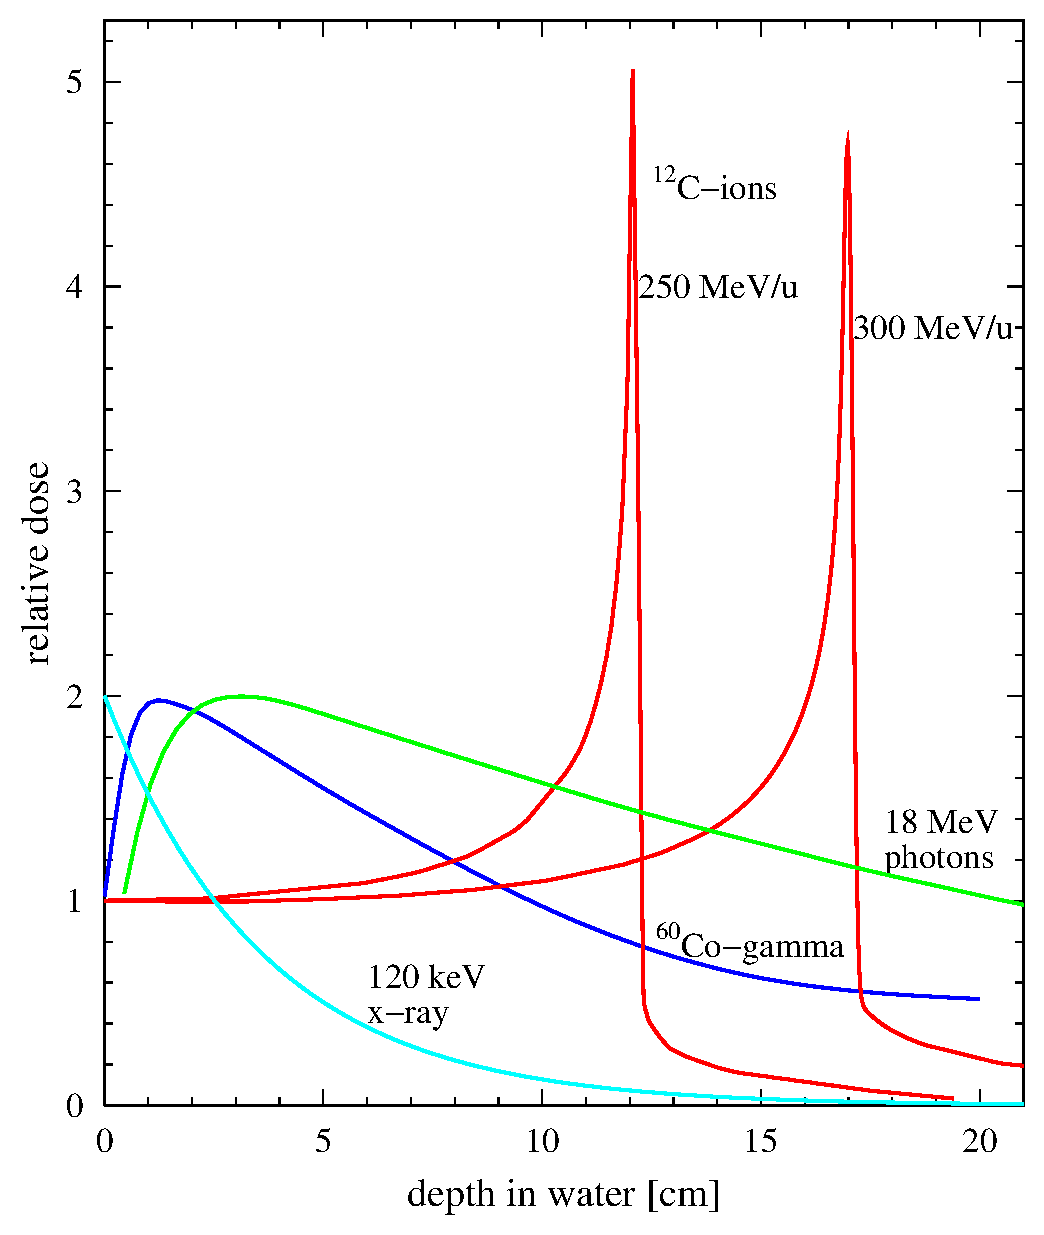
\includegraphics[scale=0.7]{./teile/introduction/depthdose.eps}
\caption{Depth dose distributions of photons and carbon ions at different energies. Photons display an exponential decrease after a certain 
build up. Ions on the other hand interact differently with matter, resulting in an increased dose deposition at the end of the particle 
track, the Bragg peak. Figure taken from \cite{Sch10}}
\label{ddp}
\end{center}
\end{figure}
% \newpage

\newpage

\subsubsection{Interaction of photons with matter}

Photons undergo different processes when passing matter, like coherent scattering or Rayleigh scattering, photoelectric effect, Compton 
scattering and pair production. The probability for each process depends on one hand on the energy of the primary photons as well as on the 
atomic number of the absorbing material, while the strength of these dependencies varies in turn on the different processes \cite{Lil06}. 
The overall decrease of the photon beam intensity when passing a material can be described by the following formula:

\begin{equation}
 I = I_{0} \cdot e^{- N \sigma x} = I_{0} \cdot e^{-\mu x}
 \label{expdecrease}
\end{equation} 

where $I_{0}$ represents the intensity of the incident photon, $x$ the depth of the material in units of length, $N$ the atomic density 
of the material and $\mu$ is the attenuation coefficient. The latter is directly related to the overall cross section $\sigma$, which is a 
measure of the probability of the occurrence of an interaction mechanism. It has contributions from all single interaction processes. 

\begin{equation}
{\sigma} = \sigma_{\mathrm{rayleigh}} + \sigma_{\mathrm{photoelectric}} + Z\sigma_{\mathrm{compton}} + \sigma_{\mathrm{pairproduction}} 
\end{equation}

In the energy range of radiotherapy (between 100 keV and 25 MeV) the dominating process is Compton scattering \cite{Alp98}. 
The attenuation of the photon beam results thus in the following way: 
The Compton electrons are scattered in a strongly forward direction, leading to a build up effect in deeper layers of the material. The 
maximum of the depth-dose profile is reached when the electrons are completely stopped at a certain depth, which is called the mean electron 
range (and is dependent on the initial photon energy). Afterwards the dose deposition decreases exponentially (see eq. \ref{expdecrease}). 


\subsubsection{Interaction of ions with matter}

Interaction of ions with matter occurs via one of the following processes: elastic coloumb scattering from target nuclei (nuclear stopping) 
and inelastic collision with target electrons (electronic stopping). In the mildly relativistic region used in radiotherapy 
(energies of less than 500$\mathrm{MeV}/\mathrm{u}$) the total stopping power of ions is dominated by electronic stopping, 
resulting in ionization and excitation of the target atoms. 
The Bethe-Bloch formula \cite{Bet30, Blo33}, describing the mean rate of energy loss of relativistic ions, can thus be corrected 
for low particle energies \cite{Nak10}, resulting in the following approximation:

\begin{equation}
- \left \langle \frac{dE}{dx} \right \rangle = \frac{ 4 \pi N_{e} z_{eff}^{2} }{ m_{e} v^{2} } \left( \frac{e^{2}}{4\pi \epsilon_{0}} \right) ^{2} \left[ln \left( \frac{2m_{e}v^{2}}{I} \right) + \mathrm{correction} \right]
 \label{bethe}
\end{equation}

where $N_{e}$ is the materials electron density, $e$ and $m_{e}$ are the charge and mass 
of an electron, $\epsilon_{0}$ the electrical field constant and $I$ the mean excitation energy of the absorber material. The effective 
projectile charge $z_{eff}$ can be approximated by the Barkas formula \cite{Bar63}, where $\beta$ is the projectile speed in units of 
$c$: 

\vspace*{-0.8cm}
\begin{equation}
 z_{eff} = z \left( 1 - e^{-125 \beta z^{\frac{2}{3}}} \right)
\end{equation}

The main dependencies of the mean rate of energy loss can be seen in equation \ref{bethe}. It is proportional to $z_{eff}$ 
and inversely proportional to $v^{2}$. The overall depth dose distribution can thus be understood in the following way: in the beginning 
the particles have a high energy and thus high velocity, causing the dose deposition to be small. While passing the material, the velocity 
of the projectile decreases, causing the energy deposition to increase. At low particle energies, close to the particle range, 
target electrons are collected hence causing $z_{eff}$ to decrease, leading to a decrease in dose deposition. The position of the maximum 
specific energy loss around the particle range is known as Bragg peak. 

\subsubsection{Range straggling and lateral scattering}
\label{scat}
Even though electronic stopping via inelastic collisions with target electrons is the main interaction process in the therapeutic energy 
range, elastic Coulomb scattering from target nuclei is still occurring and represents the main reason for lateral scattering. In an analytical 
approximation by Moli\`{e}re \cite{Mol48}, the angular spread of the overall deflection in a material has been described. It is 
on one hand dependent on the mass of the target nuclei, where a higher mass causes a larger angular spread for the same material thickness. 
And on the other hand it is inversely proportional on the momentum of the projectile, causing carbon ions to have a smaller 
lateral deflection than e.g. protons. Experimental validation comparing carbon ions to protons having the same range in water 
(15.6cm, 150MeV protons and 285MeV/u 12C ions) resulted in an approximately three times smaller angular spread \cite{Sch10}.\newline
\newline
Range straggling is caused by the statistical fluctuations of single electronic stopping events. In case of large number of collisions or 
thick layers of material these fluctuations can be approximated by a Gaussian probability distribution \cite{Bor40} 
\cite{Ahl80, Ric12}. This leads to an inverse proportional dependence between the ratio of the straggling width $\sigma_{R}$ with 
the mean range $R$ and the square root of the ion mass $M$ ( $\mathrm{\sigma_{R}}/\mathrm{R} \propto \mathrm{1}/{\sqrt{M}}$ ). This results 
in a smaller range scattering for heavier ions. Experimentally, the ratio between the straggling width and the mean range was found to be 
3.5 smaller for carbon ions compared to protons \cite{Sch10}.


\subsubsection{Nuclear fragmentation}
\label{intro:nt}
At large penetration depths, when the projectile ions have lost most of their energy, projectile fragmentation processes start to be 
relevant for ions heavier than protons. Mostly lower Z fragments are produced, which move with approximately the same velocity 
and in the same direction as the primary ions. This causes dose tails behind the Bragg peak position (see figure \ref{int:frag:fig}). 
Thus the resulting depth-dose distribution is actually the sum of the energy deposition of the projectiles and the resulting 
fragments. 

\begin{figure}[H]
\begin{center}
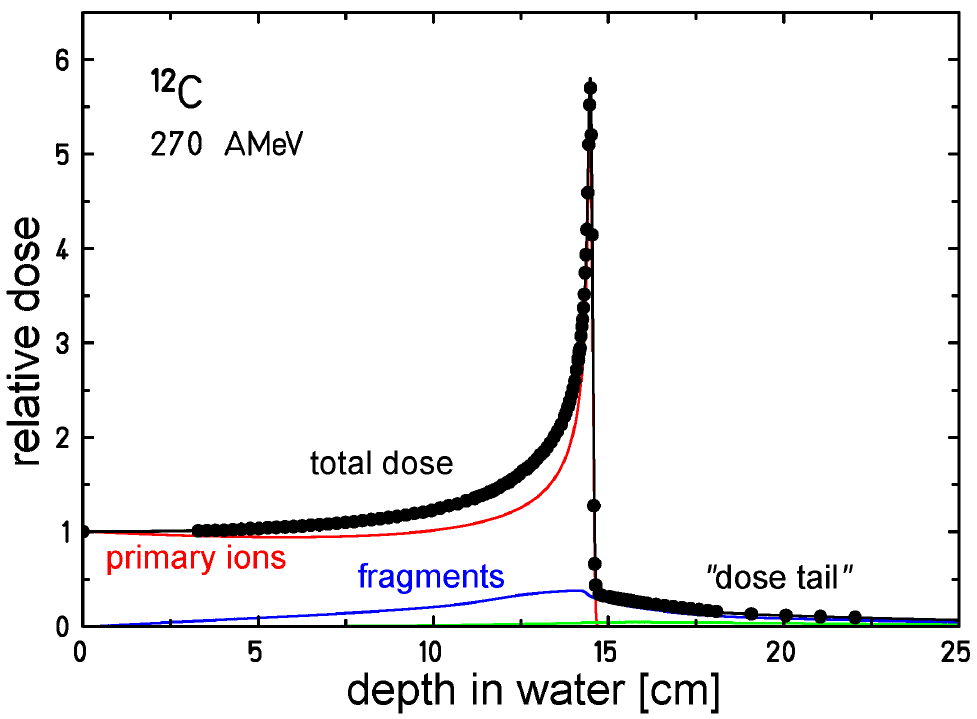
\includegraphics[scale=0.3]{./teile/introduction/iondepthdosesum.png}
\caption{Depth dose distribution of carbon ions. Besides of the energy deposition of the primary ions (red), the produced fragments 
(blue curve) contribute to the overall dose deposition (black) and are especially visible in the dose tail behind the Bragg 
peak. Figure taken from \cite{Gro04}}
\label{int:frag:fig}
\end{center}
\end{figure}

Nevertheless, the produced fragments  also offer the chance for PET (Positron Emission Tomography) monitoring, 
without additional radiation exposure for the patient. As peripheral collisions are more frequent then central ones \cite{Kra00} 
isotopes like $^{11}C$ and $^{10}C$ are often produced when $^{12}C$ ions penetrate through tissue. Both isotopes are $\beta^{+}$ 
emitters. They annihilate with electrons in the human body, producing two $\gamma$-rays which travel in opposite directions.

% \newpage

\subsubsection{Track structure}

For inelastic collisions with atomic target electrons, only about 20\% of the initial projectile energy is used to overcome the 
electron binding energy \cite{Kra92}. A high amount of energy is transformed into the kinetic energy of the secondary electrons, the 
so-called $\delta$-electrons. These $\delta$-electrons can in turn emerge from the primary particle trajectory and undergo frequent 
elastic and inelastic scattering. If their energy is sufficiently high they can induce further ionization in more distant locations, 
leading to a high number of additional electrons. The radial dose fall off is approximated by a $\mathrm{1}/\mathrm{r^{2}}$ law, 
illustrating that the radial dose quickly falls off with larger radial distance $r$ \cite{Cha76, Kat99, Ric12}. 
The range of the $\delta$-electrons is restricted to a maximum value according to the kinematics of the collision between projectile 
and target electron. Empirically this can be described by a power law \cite{Kie86}, where $E$ is energy of the primary ion:

\begin{equation}
 r_{max} \propto E^{1.7}
\end{equation}

As stated by the Bethe equation (\ref{bethe}), the energy deposition of the primary ions is dependent on the used ion species and their 
energy. This results in a higher stopping power for higher $Z$ primary ions as well as an increased stopping power for smaller energies. 
Hence carbon ions have a much higher $\delta$-electron output than e.g. protons. Furthermore with decreasing energy of 
carbon ions, the $\delta$-electron output increases. This can be seen in figure \ref{track}. The higher ionization density produced by 
$\delta$-electrons is also the reason for the difference in induced biological damage. 

\subsubsection{Linear Energy Transfer LET}


The critical measure for the energy deposition of the $\delta$-electrons is the linear energy transfer (LET). 
It is defined as the locally deposited energy to the medium (average energy deposited per unit length of track \cite{Hal06}) and 
in radiobiology is given in keV/$\mu$m. Sparsely ionizing radition (such as photons, protons and fast ions) have a low LET, while slow ions 
are densely ionizing and hence have a high LET. 


\newpage

\vspace*{1cm}

\begin{figure}[H]
\begin{center}
% 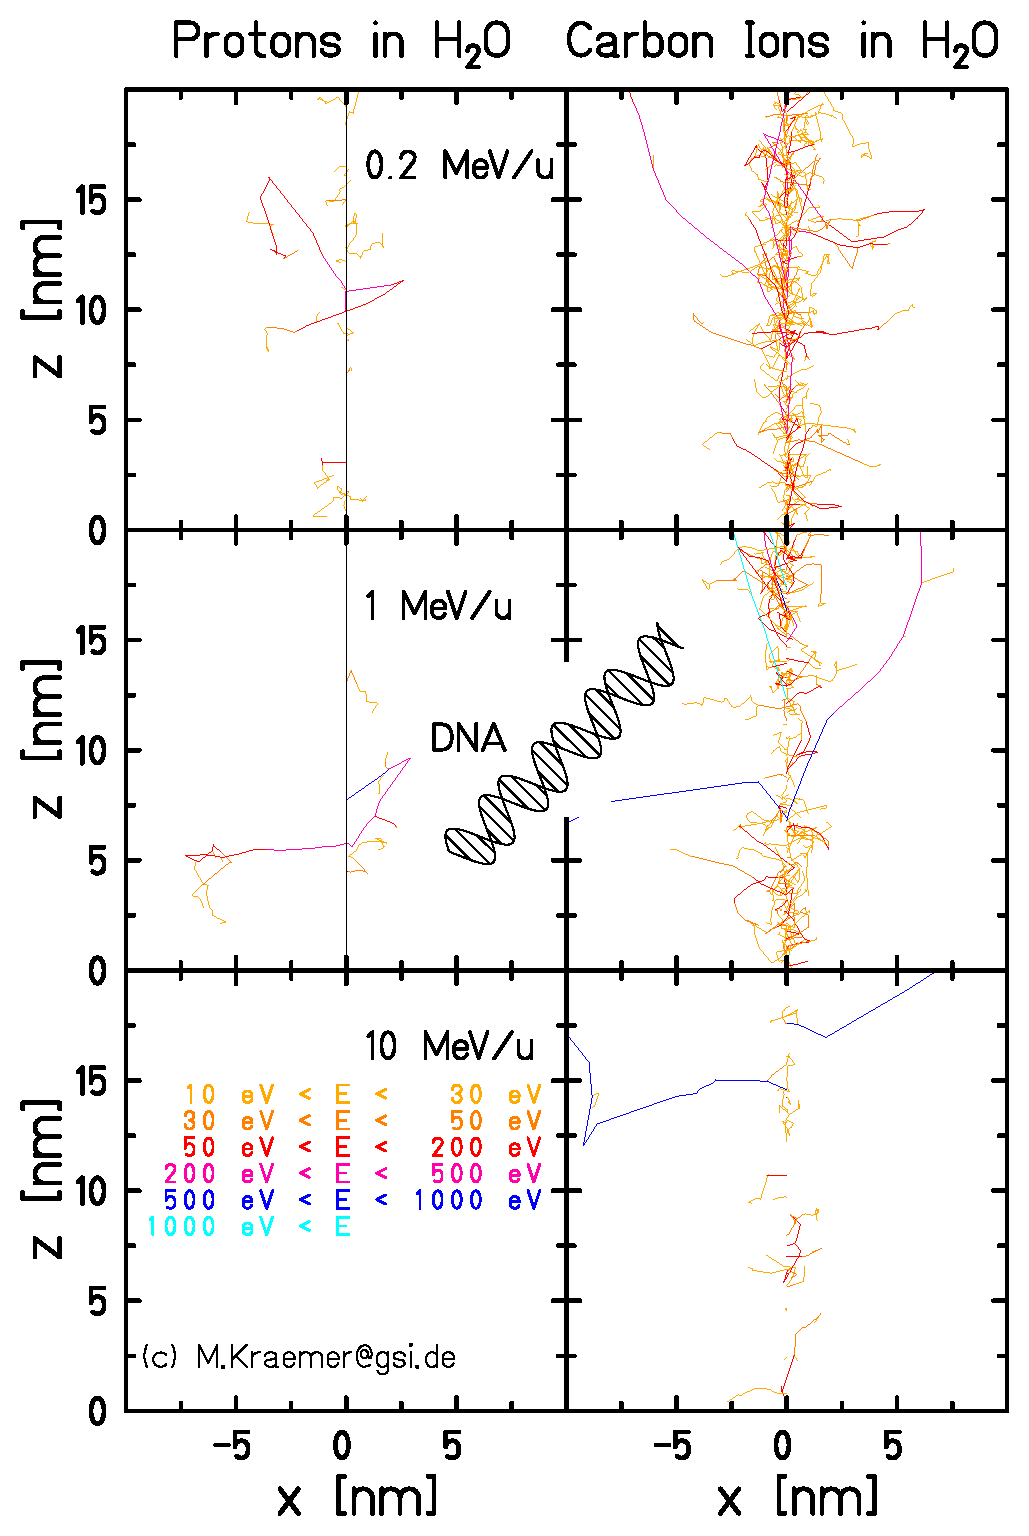
\includegraphics[scale=0.75]{trackstructure.eps}
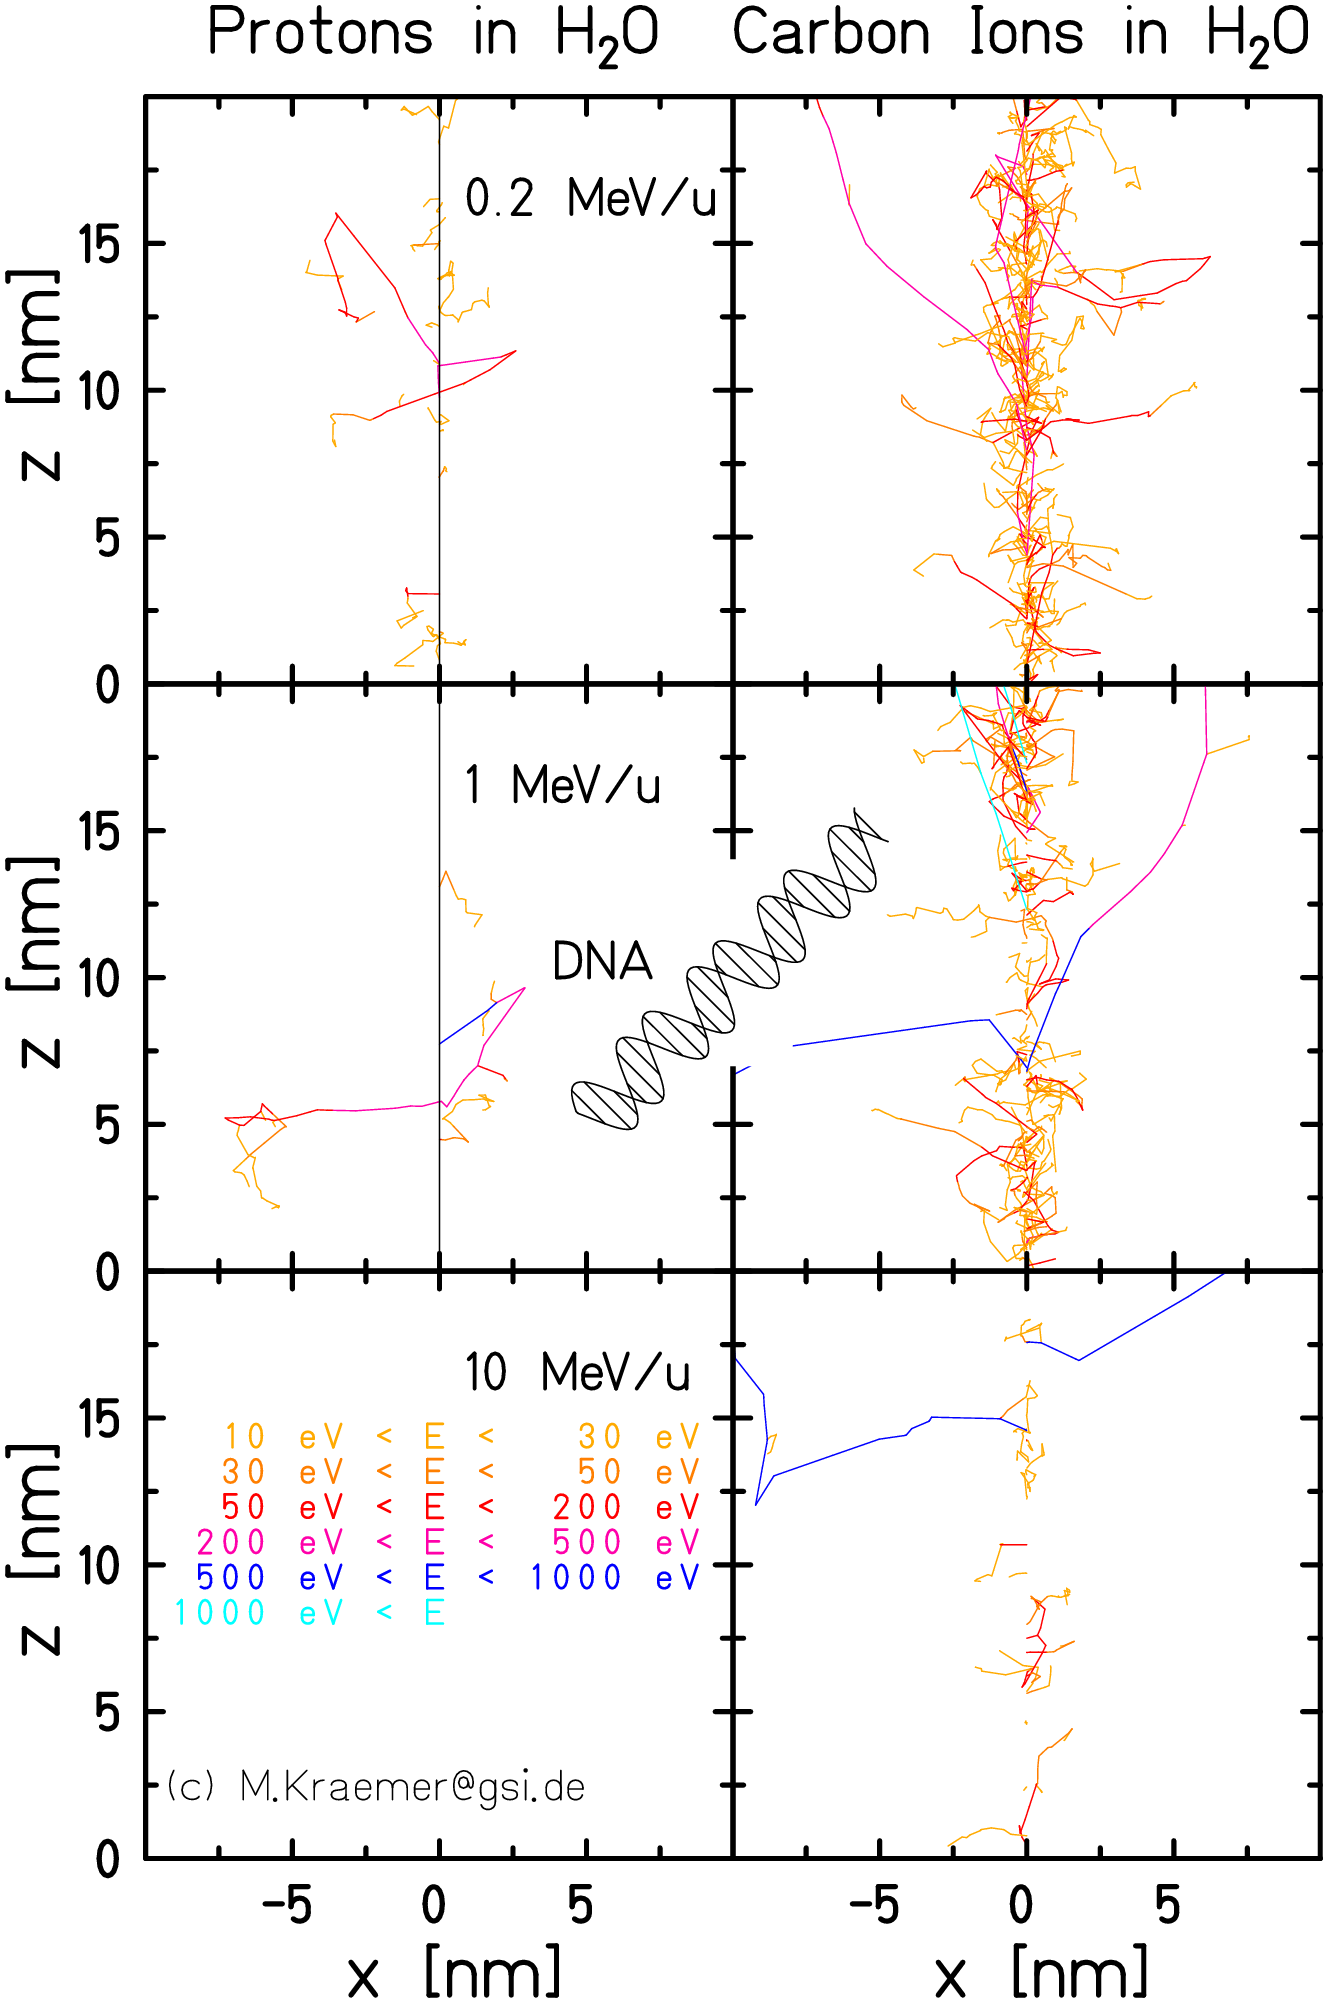
\includegraphics[scale=0.25]{./teile/introduction/trackstructure.png}
\caption{Microscopic track structure of protons (left side) and carbon ions (right side) at different energies. Protons and high energy 
carbon ions are low LET radiation and hence sparsely ionizing. Low energy carbon ions on the other hand are high LET radiation and hence 
densely ionizing. For comparison the size of the DNA is displayed. Figure courtesy of Michael Kr\"amer.}
\label{track}
\end{center}
\end{figure}



\subsection{Radiobiology}
\label{radiobio}
It was described in the previous section that both, photons and ions, are ionizing radiation producing $\delta$-electrons which 
in turn can cause subsequent ionizations. These ionizations attack the carrier of the genetic information, the DNA, of the irradiated 
cells and hence causes them to stop to proliferate. The biological background of these processes will be described in this section. 
Furthermore the enhanced biological effect of ions compared to photons will be explained. This is one of the potential benefits expected 
from a non-invasive irradiation of atrial fibrillation with carbon ions compared to photons. 


\subsubsection{Impact of radiation on cells}

In eukaryotic cells, meaning cells that contain a cell nucleus, the genetic information is stored in the DNA (desoxyribonucleic acid), 
making it therefore the critical target in radiotherapy. DNA is made of two sugar and phosphate backbones and four different base pairs 
(adenine A, cytosine C, guanine G and thymine T), which bind in a defined way (A with T and C with G) and thus form the double helix 
structure with a distance between the two strands of about 2 nm. The genetic information is encoded in the sequence of the base pairs. 
Ionizing radiation can destroy the described structure of the DNA, either by direct or indirect action \cite{Hal06}.\newline
\newline
As can be seen in figure \ref{ida} direct effects are caused by the destruction of molecular bonds of the DNA itself 
through any form of radiation. This process is considered the dominant effect if radiation with a high LET is used. Indirect action means 
that free radicals are produced by the ionizing radiation, which then in turn can damage the DNA. 
This phenomenon is predominant when sparsely ionizing radiation (low LET, like photons) are used and interact with molecules in the cell, 
particularly water.\newline
\newline
Both mechanisms can cause either single strand breaks (SBS) or double strand breaks (DSB) (see figure \label{ida}). SSB means that only 
one of the strands is destroyed, leaving the complementary base on the other strand intact and thus enabling a fast repair if the SSBs 
occur at a certain distance from each other. DSBs or clustered SSBs are more complex and can cause the breakage of the chromatin. But even 
these damages are usually steadily repaired. The repair mechanisms only start to fail when the DSBs accumulate to local lesions. Changes 
in the original DNA material is the result. Depending on the produced damage mutations, carcinogenesis or cell death can be the 
result. Cell death can occur in different pathways. Apoptosis is the controlled self-inactivation of the cell due to DNA damage and the preferred 
pathway in radiotherapy. Uncontrolled cell death, necrosis, typically causes severe reactions of the immune system, leading to e.g. 
inflammation.

\begin{figure}[H]
\begin{center}
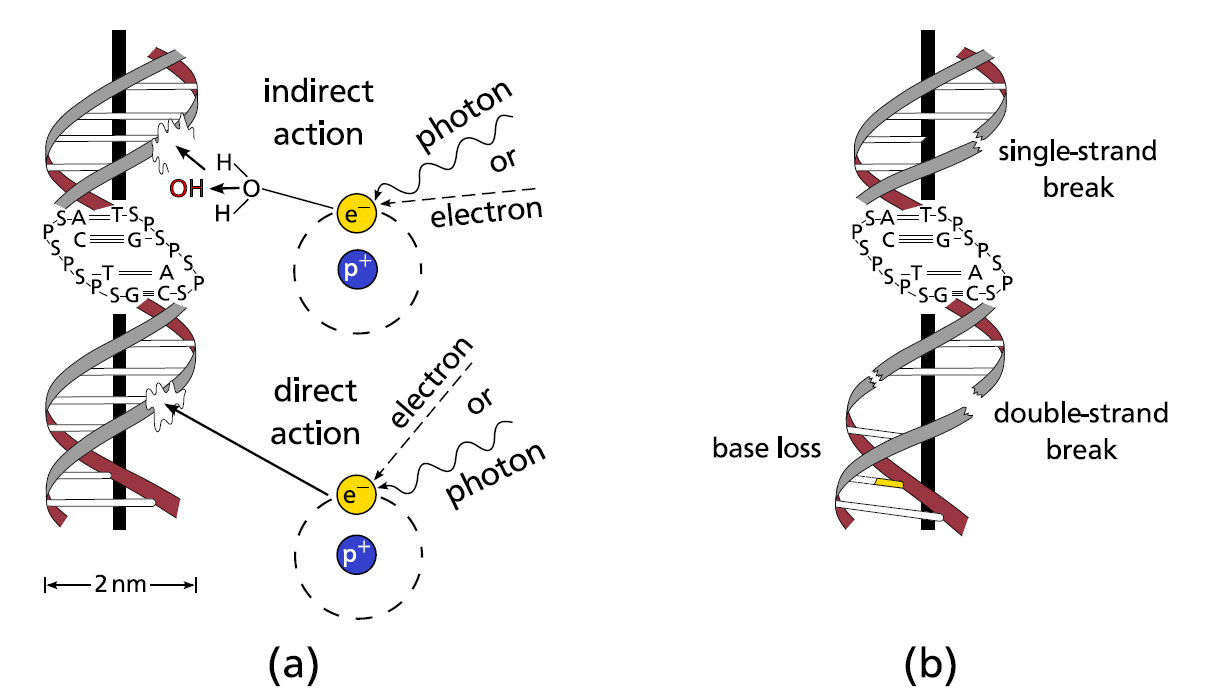
\includegraphics[scale=0.5]{./teile/introduction/SSB_DSB.png}
\caption{On the left side (a) direct and indirect radiation damages are illustrated. On the right side (b) single strand breaks and 
double strand breaks are visualized. Figure taken from \cite{Ric12}}
\end{center}
\label{ida}
\end{figure}



\subsubsection{Relative Biological Effectiveness RBE}

As outlined, at the same dose level radiation the damage depends on the LET.  This means that the induced biological effect 
is, amongst others, dependent on the energy and type of radiation. This is described in the relative biological effectiveness (RBE), 
which is defined as follows:

\begin{equation}
 RBE = \left.\frac{D^{ref}_{photon}}{D_{ion}} \right|_{\mathrm{isoeffect}}
\end{equation}

$D^{ref}_{photon}$ is the absorbed photon dose necessary to induce a certain isoeffect and $D_{ion}$ is the absorbed dose of ions at a 
defined energy which leads to the same effect. Comparison of RBE values are valid only for the same effect and biological endpoint 
and by using the same reference radiation. This idea is used in the local effect model (LEM) at GSI for the prediction of the RBE. By 
assuming that the biological effect is independent of the specific radiation type but rather dependent on the energy deposition distribution 
in small sub volumes of the cell nucleus, RBE predictions are computed in relation to the known biological response of photons 
\cite{Krae03, Fried13}. Weighting the physically absorbed dose with the RBE results in the biological dose in units of Gray equivalent 
(GyE). \newline
\newline
The RBE depends on multiple parameters, like the endpoint, the irradiated tissue and its repair mechanism, the particle type, 
the used dose level and the LET. The dependence between RBE and LET is illustrated in figure \ref{rbe_let}. In case of x-rays (sparsely ionizing) 
the probability of an induced DSB is low and in general more than one track would be required to induce DSBs, resulting in a small RBE. 
Irradiation with a LET around 100keV/${\mu}$m on the other hand is optimal in producing a biological effect, as the 
density of ionization coincides with the diameter of the DNA double helix of about 2nm. Thus radiation with this LET has the 
highest probability to induce a biological damage with DSBs. More densely ionizing radiation (LET > 200keV/${\mu}$m) produces many DSBs, 
leading to ionization events which are closer together than needed. The RBE consequently decreases again, an 
effect known as overkill effect. 

\begin{figure}[H]
\begin{center}
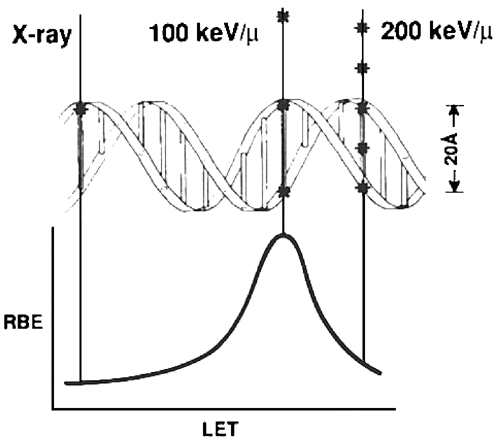
\includegraphics[scale=0.5]{./teile/introduction/rbe_let.png}
\caption{Photon radiation with a LET of 100 keV/${\mu}$m has the biggest RBE for cell killing due to the fact that average separation between 
ionizing events coincides with the diameter of the DNA double helix (2 nm). Figure taken from \cite{Hal06}}
\label{rbe_let}
\end{center}
\end{figure}

Concerning the increased biological effectiveness of ions it can be stated that it is only of advantage if the RBE is more pronounced 
in the target tissue compared to the normal tissue in the entrance channel. While protons exhibit an almost constant RBE throughout the 
energy deposition (a constant value of RBE = 1.1 is used), for ions heavier than oxygen the location for the highest RBE moves towards the 
proximal region of the depth-dose profile, starting to coincide with the plateau region \cite{Kra00}. For carbon ions on the other hand 
the position of the highest RBE value coincides with the Bragg peak region, enhancing the possibility of a beneficial treatment outcome. 



\newpage

%%%%%%%%%%%%%%%%%%%%%%%%%%%%%%%%%%%%%%%%%%%%%%%%%%%%%%%%%%%%%%%%%%%%%%%%%%%%%%%%%%%%

\section{Radiotherapy}

The conventional method for radiotherapy remains the irradiation with photons. Nevertheless, the biological and physical properties of ions 
(which were described in the previous section) result in advantages for radiotherapy, especially when treating deep seated targets. 
As a result, more and more ion facilities are opened worldwide, treating an increasing number of patients with protons and carbon ions \cite{Loe13}. 
In this section the state of the art in treating static tumors with photon and carbon ion therapy will be summarized. 
Afterwards organ motion and the resultant difficulties, as well as approaches for motion mitigation will be presented. 

\subsection{Photon therapy}

As can be seen in figure \ref{ddp}, a treatment of deep seated targets with photons can be carried out more effectively the higher the photon 
energy. Over the decades, different photon emission techniques were developed which allowed for higher photon energies. 
Currently, photons in the energy range of (6-25)MeV \cite{Ber06} are used. The photons are produced with the help of linear accelerators, which 
are used to shoot accelerated electrons on a target, thereby emitting bremsstrahlung which is then used for radiotherapy.\newline
\newline
Not only the used photon energy spectrum but also the application techniques developed over the last decades \cite{Buc05}. Two dimensional (\textbf{2D}) 
radiotherapy was based on radiographies and was carried out with a single beam, which was applied from one to four different directions, 
usually as opposing lateral fields. As the imaging techniques advanced the treatment became also more conformal. CT scans enabled axial anatomy 
and tumor visualization in three dimensions. Hence in three dimensional conformal radiotherapy (\textbf{3DCRT}) more accurate dose calculations 
with homogeneous fields are possible, leading to an increased normal tissue sparing. With the development of \textbf{IMRT} (intensity 
modulated radiotherapy) the normal tissue sparing could be further improved. In IMRT a varying number of beams 
from different beam directions are overlaid while modulating the intensity of radiation within each field. This intensity modulation is 
achieved by using multileaf collimators (MLC) (see figure \ref{lamellen}). An exemplary IMRT treatment plan in comparison to carbon ion 
irradiation can be seen in figure \ref{targetvergleich}. 

\vspace*{-0.3cm}

\begin{figure}[H]
\begin{center}
% \includegraphics[scale=0.28]{lamellen.png}
\includegraphics[scale=0.2]{./teile/introduction/lamellen.png}
\caption{Technical realization of IMRT by using multileaf collimators (MLC), enabling a photon dose deposition conformal to the 
target volume. Each lamellae can be moved individually, enabling an intensity modulation. Figure taken from \cite{Schl01}}
\label{lamellen}
\end{center}
\end{figure}


\subsection{Carbon therapy}

As already explained in section \ref{pbb} ions display an inverse depth-dose profile and a higher biological effect compared to photons. 
This enables a high target conformity and a sparing of normal tissue, both of which are beneficial for radiotherapy. 
Since 1954, when the first ion beam therapy was carried out with protons at Berkeley Lab \cite{Tob58} different projectile ions were 
used and their effect on target tissue studied.\newline
\newline
Due to the their higher momentum and thus smaller lateral scattering (see section \ref{scat}) the usage of heavy ions (heavier than protons) 
enables a better sparing of normal tissue and organs at risk (OAR), even if they are close to the target volume. 
In contrast to other ion types, the increased biological effectiveness of carbon ions  coincides with the Bragg peak region (see section 
\ref{radiobio}). Thus both the physical and biological properties of carbon ions offer the possibility of a beneficial treatment outcome. 

\subsubsection*{Application technique}

As in photon therapy, ion therapy application and thus target conformity improved over the decades after first treatments at Berkeley 
were performed by shooting the proton beam through the complete patient head \cite{Tob58}. Depending on the provided accelerator as well 
as on the beam line properties passive and active techniques are distinguished both in beam delivery as well as beam shaping.\newline
\newline
Concerning \textbf{beam delivery} particle acceleration to the therapeutic energies of several hundred MeV/u is carried out in cyclotrons and 
synchrotrons. \textbf{Cyclotrons}, which are used mainly in proton centers, offer the advantage of a more compact design compared to synchrotrons 
and allow a continuous beam extraction with stable intensities. On the other hand no active energy variation is possible, requiring the need 
for passive energy degraders. \textbf{Synchrotrons}, which are used in heavy ion centers, allow active energy variation.\newline
\newline
Concerning \textbf{beam shaping} methods, which are used in order to deposit a homogeneous dose in the target volume, \textbf{passive methods} 
are used in some carbon ion centers as well as in the majority of proton centers. The devices rely on three different beam shaping steps 
\cite{Chu93}. Firstly the beam is broadened by scattering and then further widened by using range modulators like e.g. a 
ridge filter. Thereby an extended and flat, but still homogeneous, field is formed which covers the tumor extent in longitudinal direction 
(Spread Out Bragg Peak: SOBP). Secondly, the range adjustment of the SOBP is achieved via flat degraders of variable thickness. Final 
conformity to the distal target border is achieved by patient individual compensators. Collimators are used for a lateral 
conformity. A scheme of a passive beam shaping system can be seen in figure \ref{passive}. Passive beam shaping devices offer the benefit 
that the historically unstable beam quality of research facilities - in which the first treatments were carried out - did not influence the 
homogeneity of the applied dose. Moreover, beam energy changes during treatment can be avoided, thus enabling a fast irradiation time. 
Nevertheless, passive beam application always requires the manufacture of patient individual compensators and an unavoidable limitation in 
volume conformity in the proximal tumor region as the SOBP width is fixed by the range modulator to the largest needed depth (see 
figure \ref{passive}). Material in the beam path means furthermore intensity loss due to lateral scattering and an extra dose exposure 
due to fragmentation.


\vspace*{0.8cm}
\begin{figure}[H]
\begin{center}
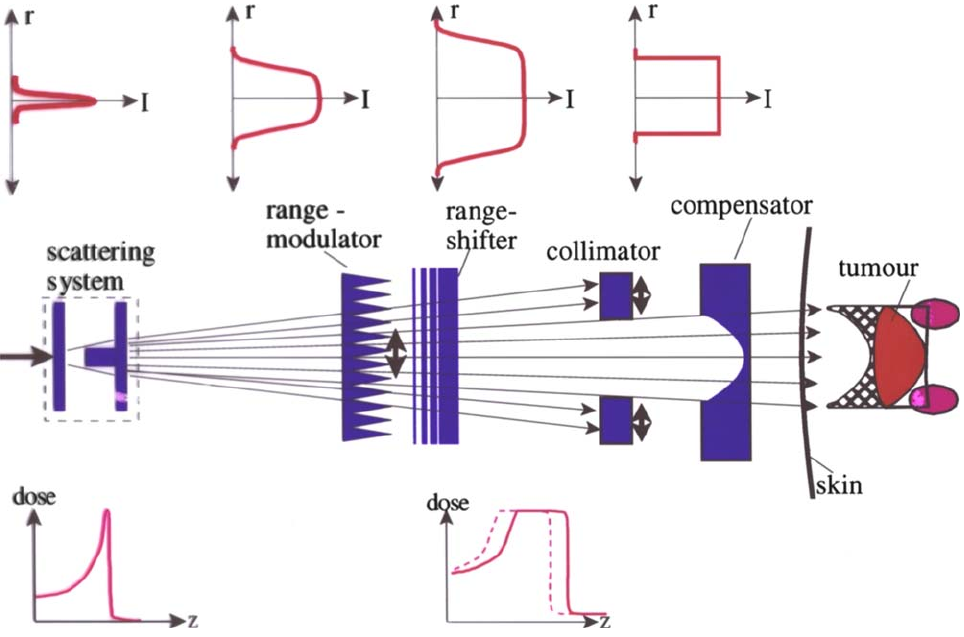
\includegraphics[scale=0.4]{./teile/introduction/deliverypassive.png}
\caption{Scheme of a passive beam shaping system. The beam is broadened by a scattering system and the width of the SOBP is determined by a 
range modulator. Via a range shifter the SOBP energy can be adjusted to a fixed range and thus depth. For lateral conformity collimators are 
used. The longitudinal conformity to the distal border of the target is achieved with a patient specific compensator. The proximal volume 
border can not be shaped, as is indicated in the hatched areas. Figure taken from \cite{Sch10}}
\label{passive}
\end{center}
\end{figure}

\newpage

\textbf{Active beam shaping} is achieved with beam scanning, which offers a very good lateral target coverage as well as volume conformity 
also in the proximal field region. The target volume is thereby subdivided into slices of the same beam energy, so called iso-energy slices 
(IES). Each IES is again subdivided into a grid of target points which are irradiated sequentially. Hence many small pencil beams are used to 
generate a conformal dose deposition to any arbitrary target volume shape without the need of patient specific hardware. This drastically 
decreases the amount of material the beam has to traverse and hence reduces the unwanted neutron dose to the patient \cite{Kad12}. Examples of 
beam scanning are spot scanning, which was developed for protons at the Paul Scherrer Institute (PSI, Swiss) \cite{Ped95} or raster scanning, 
which was developed in parallel at GSI \cite{Hab93}. \newline
\newline
At PSI a cyclotron is used and the energy variation is carried out with a degrader. The lateral deflection of the beam position is either 
achieved with magnets (Gantry 2 at PSI \cite{Ped04}) or a combination of magnets and patient couch motion (Gantry 1). The beam is thereby 
switched off between different beam positions in the order of milli seconds. \newline
\newline
Raster scanning on the other hand works in a continuous irradiation mode for one IES. A pencil beam is extracted from the synchrotron with a fixed energy and thus range, 
corresponding to a IES of the volume. By overlaying many different energies a SOBP is created to cover the longitudinal extension of the tumor 
(see figure \ref{active}b). The raster points within each IES are irradiated by deflecting the pencil beam via two orthogonal dipol magnets 
on an optimized path (see figure \ref{scanning}). When the pre-defined intensity of the raster point has been reached, the beam is moved to the next position. 
In order to establish a homogeneous dose coverage in the target volume the spacing, both in raster point position as well as IES distance, 
can be utilized. Robustness in longitudinal direction can be achieved with overlap of the individual IES slices. Nevertheless the number of 
IES slices should be kept small in order to guarantee a short treatment time. Hence a broadening of the Bragg Peak position is carried out 
with a so-called ripple filter (see figure \ref{active}b). It was found that a spacing of 3mm between IESs yields a robust result \cite{Web99}. 
Furthermore the lateral overlap of the pencil beams needs to be chosen in such a way that the possibility of minor fluctuation in beam 
quality and position is compensated for. As the lateral beam profile is assumed to be Gaussian shaped and symmetric it was found that the 
full width half maximum (FWHM) of the beam is optimally chosen to be three times the raster spacing (see figure \ref{active}a) \cite{Hab93}. 

\newpage

\vspace*{0.6cm}

\begin{figure}[H]
\begin{center}
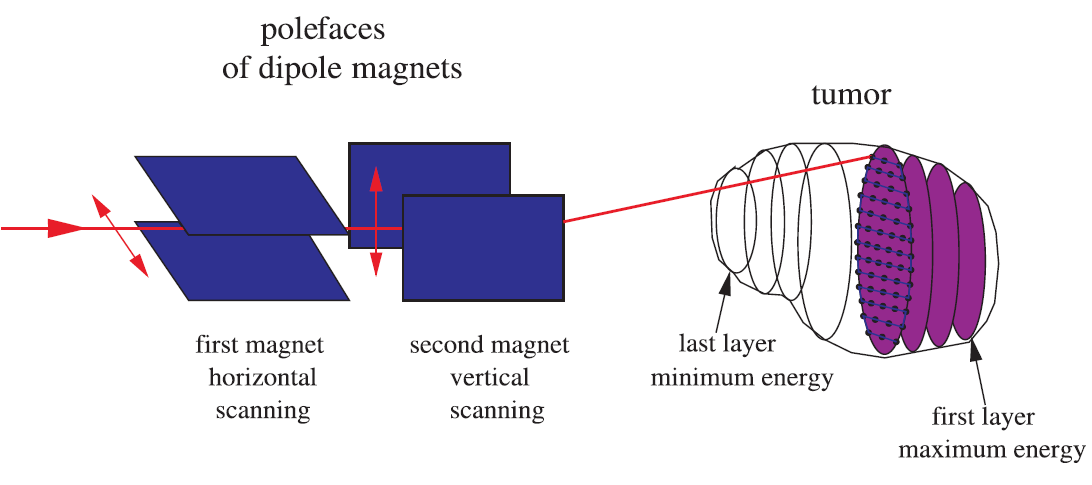
\includegraphics[scale=0.4]{./teile/introduction/therapy.png}
\caption{Principle of the raster scanning technique at GSI. The target volume is divided into IES, which is again subdivided into a regular 
grid. By varying the particle energy from the accelerator and by deflecting the pencil beam via a magnetic scanning system the raster points 
are scanned. Figure taken from \cite{Inf05}}
\label{scanning}
\end{center}
\end{figure}


\begin{figure}[H]
\begin{center}
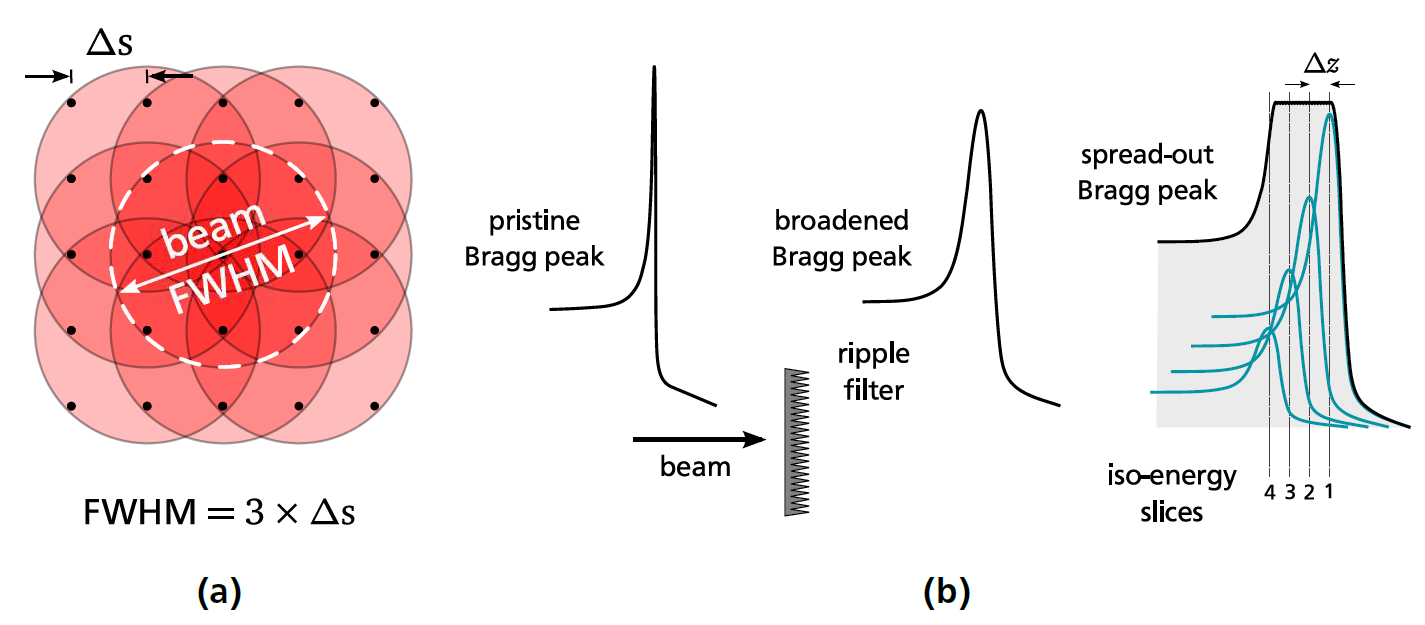
\includegraphics[scale=0.45]{./teile/introduction/active.png}
\caption{Target dose homogeneity is achieved by sufficient overlap in lateral and longitudinal directio. a) In lateral direction the FWHM of 
the pencil beam is adjusted to three times the raster spacing $\Delta\mathrm{s}$. b) In longitudinal direction the Bragg peaks are broadend 
in depth by using a ripple filter and then stacked in depth to a SOBP. An IES spacing $\Delta\mathrm{z}$ of typically 3mm is chosen. 
Figure taken from \cite{Ric12}}
\label{active}
\end{center}
\end{figure}


\newpage

\subsubsection*{GSI pilot project}

Between 1997 and 2008 440 patients were treated with scanned carbon ions at GSI. Mostly head and neck tumors were irradiated. 
The typical fractionation scheme was 20 fractions within three weeks \cite{Schu07}. An example of a resulting 
dose distribution with scanned carbon ions in comparison to IMRT can be seen in figure \ref{targetvergleich}. 
The treatment outcome for skull-based chordomas can be seen in figure \ref{chordoma}. In a later stage, also prostate and spinal cord 
tumors were treated.

\begin{figure}[H]
\begin{center}
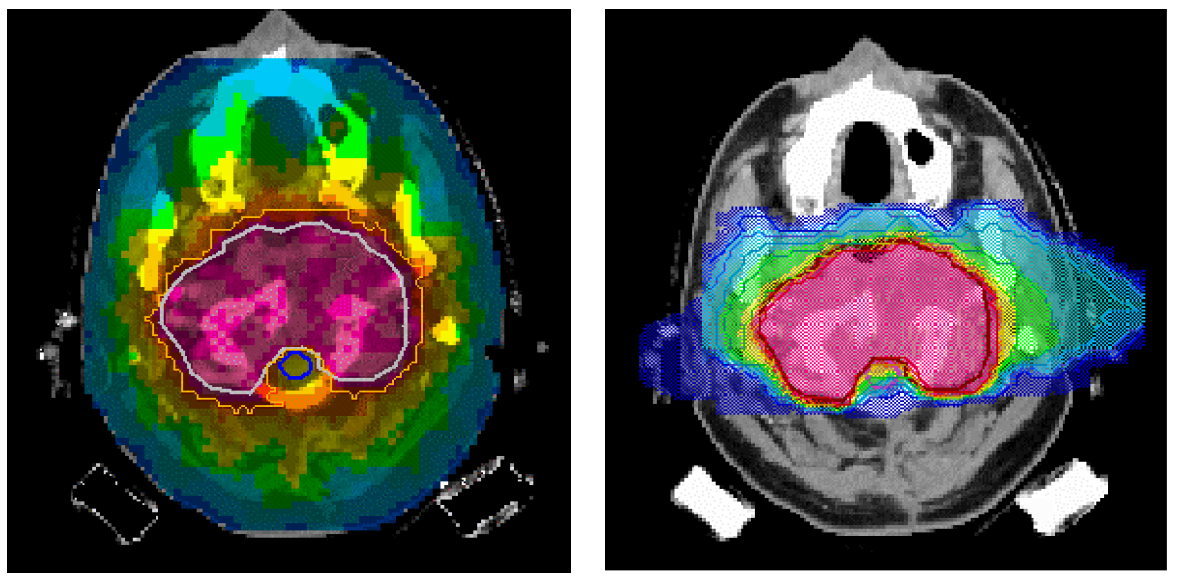
\includegraphics[scale=0.25]{./teile/introduction/targetvergleich.png}
\caption{Comparison of dose distributions results with IMRT (left side) and scanned carbon ions (right side). The dose to the normal 
tissue and especially organs at risk like the brainstem are drastically reduced for scanned carbon ions. Figure taken from \cite{Gro04}}
\label{targetvergleich}
\end{center}
\end{figure}

\vspace*{-1cm}

\begin{figure}[H]
\begin{center}
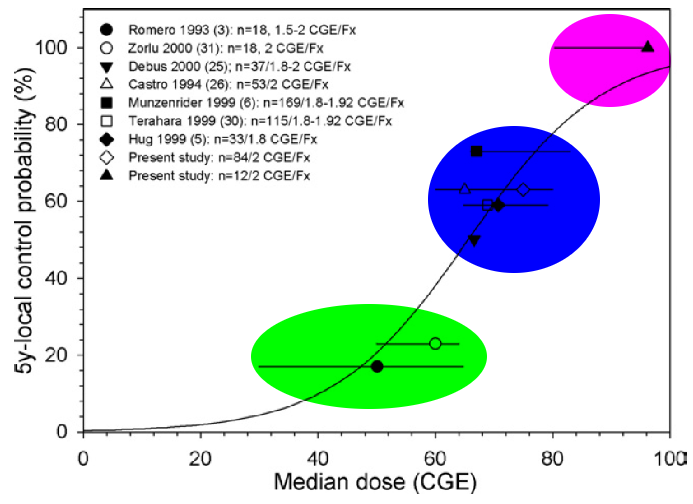
\includegraphics[scale=0.35]{./teile/introduction/chordoma_farben.png}
\caption{Treatment outcome for the irradiation of skull-based chordomas for photons (green area), protons (blue area) and carbon ions (pink 
area). An improved effect after the irradiation of chordomas can be seen when doses exceeding 70 Cobalt Gray Equivalent (CGE) can 
be applied. For carbon ions ahigher dose can be deposited in the target since the dose in the nearby OAR can be reduced. Figure taken 
from \cite{Schu07}}
\label{chordoma}
\end{center}
\end{figure}

The pilot project at GSI was carried out in a collaboration between GSI, the Heidelberg University hospital, the German cancer research 
center (DKFZ) and the research center Dresden-Rossendorf. Following the success in treatment outcome \cite{Loe13} the Heidelberg Ion-Beam Therapy 
Center (HIT) was build, where patients are treated with scanned carbon ion beams and protons on a regular basis since 2009 \cite{Com10}. 
Furthermore CNAO (centro nazionale di adroterapia oncologica, Pavia, Italy) \cite{Ama04} started treating patients with scanned carbon ions 
beams in 2012 \cite{PTCOG13}. In total roughly 10,000 patients have been treated with carbon ions up to the beginning of 2013 \cite{Loe13}, 
whereof about 2,000 patients were treated with scanned carbon ions \cite{PTCOG13}.


\subsection{Treatment planning}
\label{tp}
Treatment planning is the optimization process in which the needed machine delivery parameters are determined for a chosen beam 
configuration in order to yield the prescribed dose to the target volume, while minimising the dose to the normal tissue, ecspecially 
to the OARs \cite{Ric12}. In modern radiotherapy treatment planning is based on CT scans, which represent photon attenuation through 
the different tissue types (Hounsfield units - HU) and can hence be converted to water-equivalent depths. On the patient image data the 
target and OARs are contured and the needed dose and dose constraints, respectively, are determined. For cancer radiotherapy the delineation 
of the tumor includes certain safety margins, defined by the International Commission on Radiation units and Measurements (ICRU). As some 
of these margins will be also used in the context of cardiac targets, they will be shortly introduced here. 

\begin{enumerate}
 \item [] \textbf{GTV (Gross Tumor Volume)}: "The GTV is the gross palpable or visible/demonstrable extent and location of the malignant 
 growth." \cite{ICRU93a}
 \item [] \textbf{CTV (Clinical Target Volume):} "The CTV is a tissue volume that contains a GTV and/or subclinical microscopic malignant 
 disease, which has to be eliminated. This volume thus has to be treated adequately in order to achieve the aim of therapy: cure or 
 palliation." \cite{ICRU93a}
 \item[] \textbf{PTV (Planning Target Volume):} "The PTV is a geometrical concept, and it is defined to select and appropiate beam size 
 and beam arrangements, taking into consideration the net effect of all the possible geometrical variations, in order to ensure that the 
 prescribed dose is actually absorbed in the CTV." \cite{ICRU93a}
 \item[] \textbf{IM (Internal Margin):} "The IM, commonly asymmetric around the CTV, is intended to compensate for all movements and all 
 variations in site, size and shape of the organs and tissues contained or adjacent to the CTV. They may result e.g. from respiration, 
 different fillings of the bladder, different fillings of the rectum, swallowing, heart beat, movements of the bowel" \cite{ICRU99}
\end{enumerate}

Based on this definition, the \textbf{ITV (Internal Target Volume)} is commonly used for the volume in which the IM encompasses the CTV 
(see figure \ref{int:margins:fig}). 

\begin{figure}[H]
\begin{center}
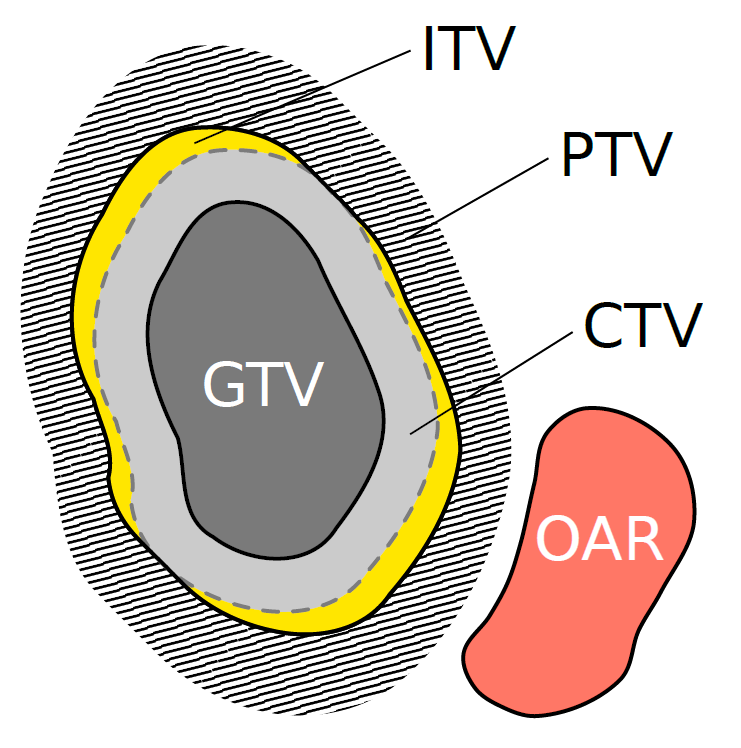
\includegraphics[scale=0.3]{./teile/introduction/volumes.png}
\caption{Treatment planning volumes as defined by the ICRU. Figure taken from \cite{Ric12}}
\label{int:margins:fig}
\end{center}
\end{figure}

\vspace*{-0.3cm}

As a result of treatment planning the ICRU recommends that 100\% of the PTV should receive at least 95\% and not more than 107\% of the 
prescribed dose \cite{ICRU93a}. In order to study if this recommendations are met, dose-volume-histograms (DVH) are computed in the 
treatment planning study process and the values V95 and V107 (the volume which receives 95\% and 107\% of the dose, respectively) determined. 
Furthermore D5 and D95, which denotes the dose covering 5\% and 95\% of the volume, are extracted. The difference between these two values 
(D5-D95) is a measure for the dose fall off and should be ideally close to zero. In general, the dose constraints of the OAR depends on the 
organ as well as fractionation scheme and radiation type and needs to be carefully examined in each individual case.\newline
\newline
The treatment planning system and its result, the dose optimization, depends on the radiation type and on the used beam delivery 
technique. For scanned carbon ion beams the optimization task with the in-house treatment planning software TRiP98 \cite{Krae00} 
\cite{Krae00b} needs to determine the required energies of the IESs and the pencil beam positions as well as corresponding particle numbers 
for each raster point. This leads to an 'inverse' optimization process, in which the particle fluence to the target volume, which is given in 
the form of planar polygon originating from manual delineation on the axial CT slices \cite{Ric13}, is determined from the prescribed dose 
distribution \cite{Kra00}. Furthermore, as the irradiation 
of the most distal IES deposits a certain dose in the more proximal slices only the distal slice 
receives a homogeneous fluence distribution while all other slices require irregular dose patterns (see figure \ref{inhomo}). Using the 
physical and biological beam models (LEM, see RBE in section \ref{radiobio}) the dose contributions from all raster points to each 
individual target voxel are calculated \cite{Ric12}. 

\begin{figure}[H]
\begin{center}
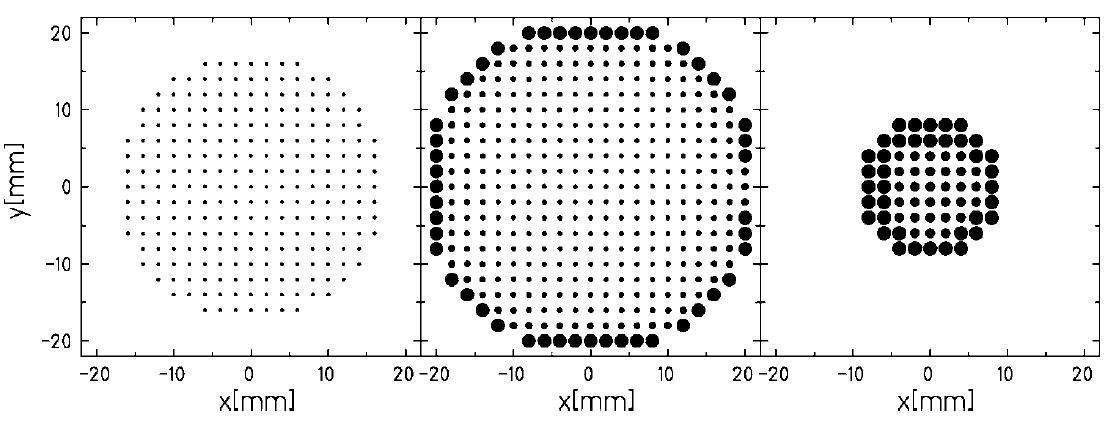
\includegraphics[scale=0.4]{./teile/introduction/inhomo.png}
\caption{Particle fluence distribution depending on the IES, starting with the most distal one (left) and moving to more proximal regions. 
Figure taken from \cite{Krae00}}
\label{inhomo}
\end{center}
\end{figure}

% \vspace*{-1cm}

\subsection{Organ motion in radiotherapy}

Many target sites are influenced by temporal changes. Depending on the underlying mechanism, one distinguishes patient positioning 
related organ motion and organ motion in-between treatment fractions (interfractional motion) or during a treatment 
application (intrafractional motion). The different organ motion types will be specified in this section. Furthermore motion acquisition 
strategies as well as techniques to overcome the motion influence, so called motion mitigation techniques, will be presented. Finally an 
overview over the treatment planning workflow including motion (four dimensional - 4D) will be given. 

\subsubsection{Motion types}

An overview of the different organ motion types is given by Langen and Jones \cite{Lan01}. Three main categories can be determined: 
patient positioning related motion, interfractional motion and intrafractional motion. Examples of these different motion types can be seen 
in figure \ref{motion}. It should be noted that all motion types can occur in a patient. Thus when dealing with intrafractional motion, 
interfractional motion as well as patient positioning needs to be accounted for.\newline
\newline
\textbf{Patient positioning} can cause changes in tumor shape as well as uncertainties in the tumor position. A difference in positioning 
between image acquisition (e.g. CT) and treatment delivery may introduce systematic displacements and hence threaten the outcome of the 
treatment. Patient fixation systems and dedicated protocols are applied to overcome this motion influence. Stereotactic fixation with e.g. 
masks are used on a daily basis. The other two motion types however are purely internal and are distinguished according to the time scale 
they occur on.\newline
% \newline
\newpage
\textbf{Interfractional motion} occurs within hours and days, hence between two treatment sessions (if multiple fractions 
are applied). Anatomical changes caused by interfractional motion are manifold. Prostate cancer patients are often subject to position 
changes due to varying gut and bladder fillings \cite{Fok04}. For lung cancer patients, changes in the breathing pattern are troublesome. 
Sonke et al. \cite{Son08} reported that even though the respiratory motion trajectory is often reproducible, the baseline of the tumor 
motion can vary significantly. Cancer patients in general are also subject to tumor shrinkage \cite{Mor09} in the course of the treatment. 
In order to mitigate interfractional motion, repeated imaging needs to be carried out.\newline
\newline
\textbf{Intrafractional motion} occurs on a time scale of seconds to minutes. The main reason for intrafractional motion are respiration 
and heart beat. Even though the exact motion patterns varies from patient to patient, it can be stated that breathing is a quite regular 
and slow process, with a rather big amplitude. Heart beat on the other hand has a smaller amplitude compared to respiration, but it is a 
high frequency motion with 60 to 80 heart beats per minute compared to 10 to 20 respiration cycles in the same time. These two motions 
superimpose and the influence of both will be studied in the framework of this work when targeting sites in the heart. Different motion 
mitigation techniques for intrafractional motion will be presented in a seperate subsection. 

\begin{figure}[H]
\begin{center}
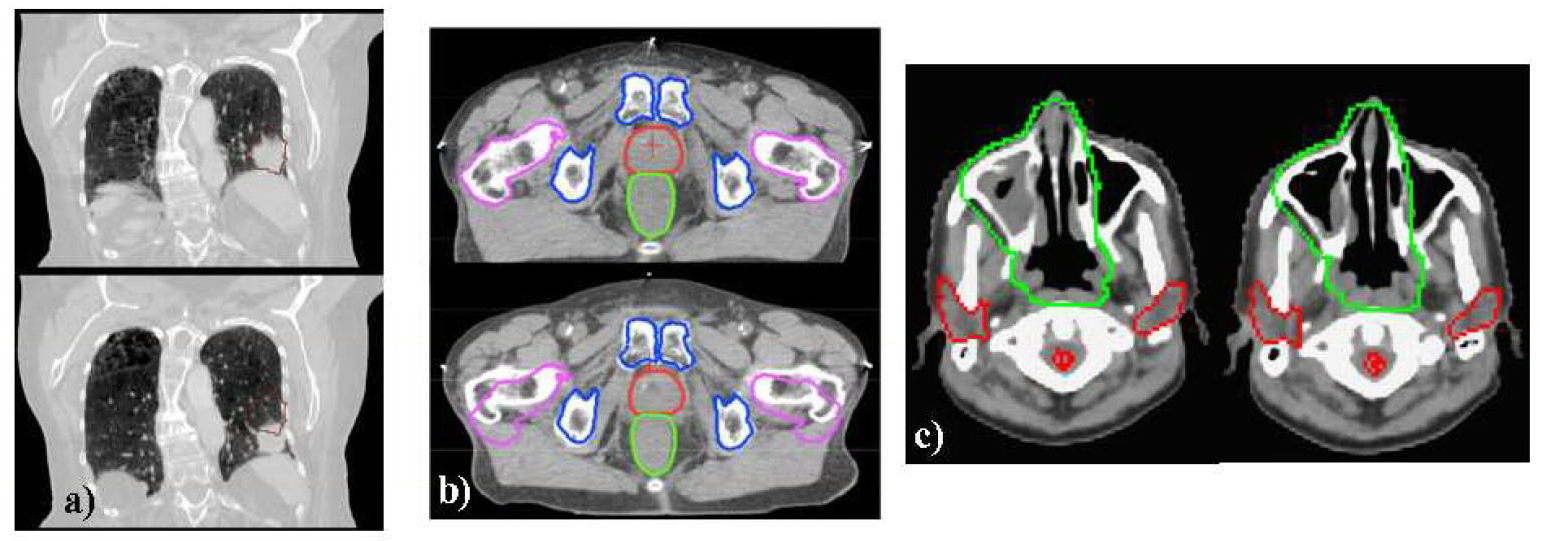
\includegraphics[scale=0.43]{./teile/introduction/motion_examples.png}
\caption{Examples of the three major motion categories. On the left side (a) a lung tumor is displayed, which moves due to the respiration 
of the patient (intrafractional motion). Interfractional position changes are examplary shown in the middle (b), where two CT scans of a 
prostate patient are compared. Density variations between two CT scans are shown in (c). Figure taken from \cite{Eng11}}
\label{motion}
\end{center}
\end{figure}

\subsubsection{Motion acquisition}
\label{Motionacq}
For a successful irradiation of the moving target, the intrafractional motion of the target site must be known during the treatment process. 
This is for example achieved by time resolved computed tomography scans (4D-CTs) and the potential usage of online motion measurement.\newline
\newline
For the acquisition of 4D-CT scans the motion signal is recorded during the imaging. The motion cycle is then divided into $N$ quasi-stationary 
sections (so-called motion phases (MP)). In every MP a full regular CT scan is reconstructed. In order to achieve this data is recorded in every 
slice for a whole motion cycle. By correlating the data gained from the motion signal with the recorded CT information, the 
scans are afterwards rearranged according to their affiliation to a certain MP. For more information on 4D-CTs the reader is refered to 
e.g. \cite{Rie05}.\newline
\newline 
A review of the different motion detection techniques can be found at \cite{Eva08}. 
One distinguishes between direct measurement techniques and surrogate signals. Examples for direct measurements are ultrasound and 
fluoroscopy. In fluoroscopy, the patient is irradiated with X-rays and the absorption pattern is displayed on a fluorescent screen, hence 
limiting the acquisition time of this method by the deposited dose. The monitoring time in ultrasound is not limited since no ionizing radiation 
is needed and hence a real time imaging is feasible \cite{Pra12}. Nevertheless influence of air limits the resolution and thus raises 
difficulties when being applied in the thorax region of the patient. Surrogate signals detect variables which are directly related to the 
source of organ motion. Examples of these kind of techniques for respiration are methods which correlate the movement of the torso to the 
phase in the respiration cycle. One possibility is to monitor the height of the patient surface with camera systems or laser 
displacement sensors or additionally using infrared markers attached to the patient's body \cite{Tad98, Ber05, Schw04, Ser13}. 
Alternatively the volume of the torso can be measured by using a belt-like strain gauge \cite{Li06}. Other approaches measure e.g. the airflow 
of the patient \cite{Kub96, Hanl99}.\newline
\newline
Combinations between direct measurement techniques and surrogate signal acquisition exist and are e.g. used in the 
Cyberknife system. Their Synchrony system (see also \ref{cardiacradiosurgery}) combines fluoroscopy (direct) with an infrared camera 
system (surrogate). This offers the advantage of a drastically reduced fluoroscopy acquisition time as it is only used to check and 
update the surrogate system \cite{Sha10, Lue12}.

\newpage

\subsubsection{Motion mitigation techniques for intrafractional motion}

% In conventional radiotherapy and passive particle therapy, moving targets are treated by enlarging the safety margins to the target region 
% (irradiating the ITV, which encompasses the target motion - see sections before). A homogenous dose distribution is thereby achieved. 
% In treatment modalities like IMRT and 
In particle beam scanning the beam delivery interferes with the intrafractional target 
motion, causing local over- and underdosages in the target volume, an effect known as Interplay \cite{Phi92, Ber08, Ber12, Loe13}. 
The exactly resulting interplay pattern is dependent on many different factors, like the beam direction, the scanning speed, the motion 
amplitude and starting phase etc. Thus techniques which mitigate the influence of the underlying target motion have to be applied. The three 
main techniques (rescanning, gating and tracking) will be explained in more detail.\newline
\newline
\textbf{Rescanning}, also known as repainting, is a specific approach for beam scanning and based on statistical averaging of different 
interplay patterns \cite{Phi92, Rie10}. Scanning the target $N$ times with a reduced dose of $\mathrm{1}/\mathrm{N}$ results in a 
Gaussian distributed dose around the theoretically intended one (see figure \ref{rescanning}). As the variance of the distribution is proportional 
to $\mathrm{1}/\mathrm{\sqrt{N}}$ the result will be better the more rescans are used. The technical realisation of rescanning is easier than 
for e.g. gating and beam tracking, 
especially as it does not require real-time motion monitoring, and results in a homogeneous dose to the inner region of the target when 
using enough rescans $N$. Anyhow it can lead to an increased dose deposition to the surrounding, normal tissue and to under dosages in 
the outer part of the target volume. So far rescanning has not been used in patient treatments, but certain centers (e.g. NIRS \cite{Fur07}) 
and PSI \cite{Zen10}) plan it for the future.

\vspace*{-0.4cm}

\begin{figure}[H]
\begin{center}
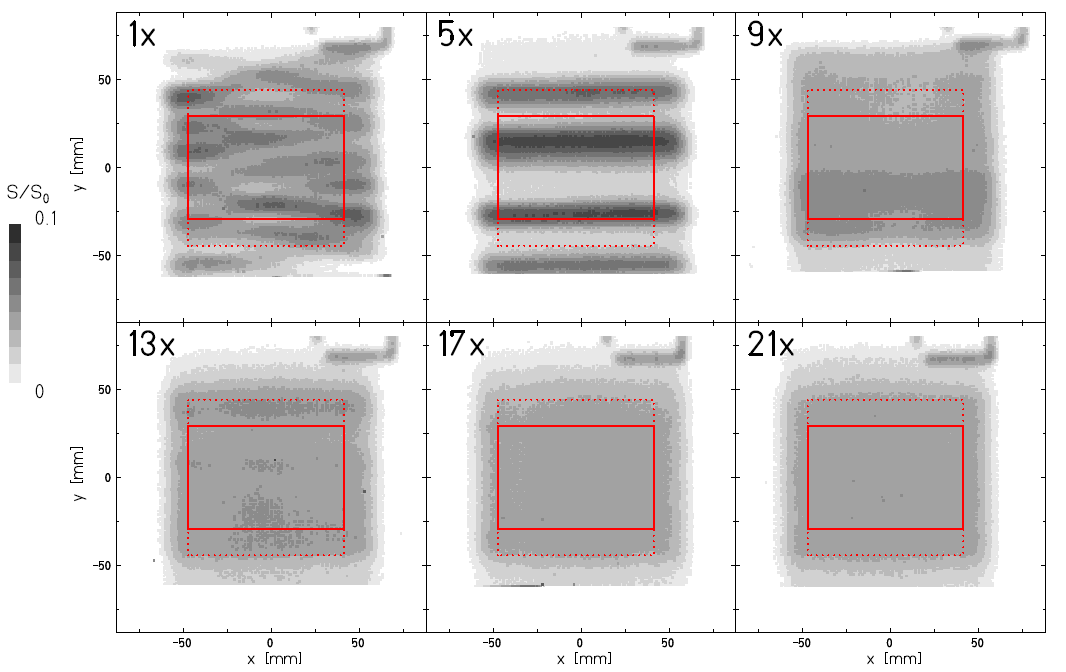
\includegraphics[scale=0.45]{./teile/introduction/rescanning.png}
\caption{Principle of rescanning in film irradiations. Averaging multiple interplay patterns leads to a homogeneous dose in the target area 
(solid red square). Figure taken from \cite{Ber09b}. }
\label{rescanning}
\end{center}
\end{figure}

\textbf{Gating} is the interrupted irradiation of the target during a selected part of the motion cycle, the gating window \cite{Kub96, Min00} 
\cite{Li06} (see figure \ref{gating}). Typically a gating window around the most reproducible motion states are chosen, which show a comparably 
small motion (e.g. end exhale in case of respiration). This technique is also used for passive beam delivery, as it reduces the size 
of ITV margins. In the gating window a small motion, the so-called residual motion, remains. In case of beam scanning this can result in 
small interplay effects. Different approaches are studied to overcome this drawback \cite{Fur07, Zen10, Ber09}. Gating requires 
online motion monitoring and prolongs the treatment time. For centers with passive beam delivery gating has already been successfully 
used \cite{Min00, Iwa10, Has06}.

% \vspace*{-0.6cm}

\begin{figure}[H]
\begin{center}
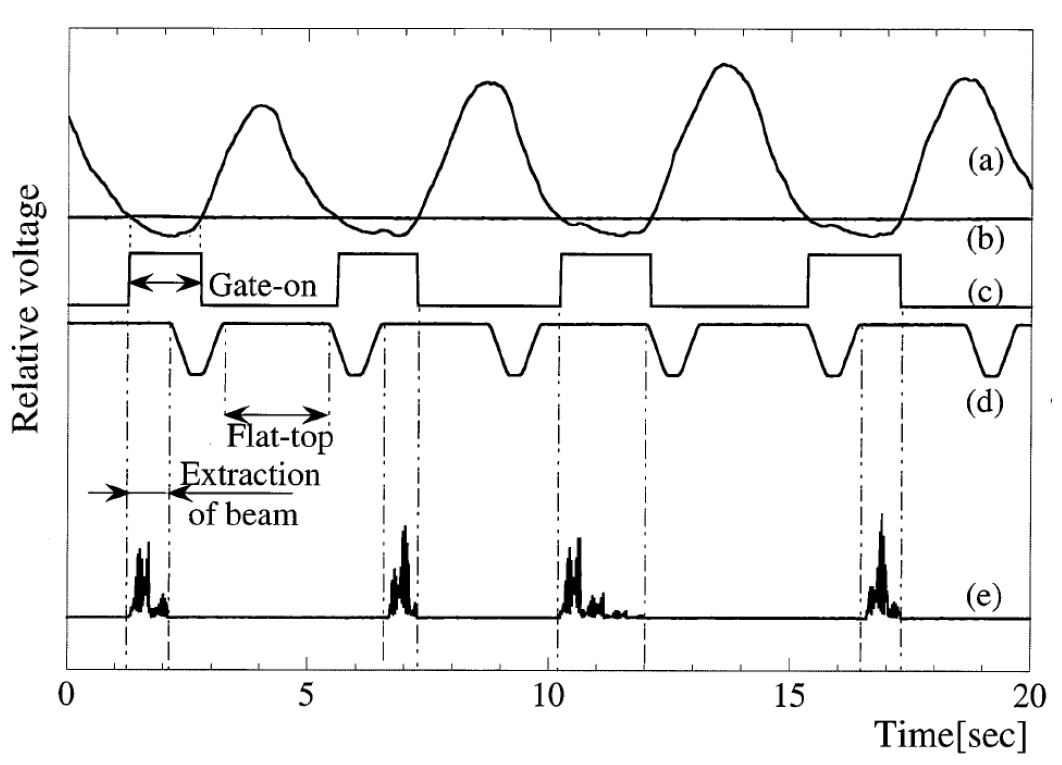
\includegraphics[scale=0.45]{./teile/introduction/gating.png}
\caption{Principle of gating. Line (a) is the respiratory signal. At end exhale the gradient of the respiration is flat, enabling an 
irradiation without large effects of the target motion. The beam (c) is thus only applied during this time. The gating window is activated 
as soon as the respiratory motion crosses line (b). Figure taken from \cite{Min00}}
\label{gating}
\end{center}
\end{figure}


\textbf{Beam tracking} of organ motion requires the adaptation of the beam position to the target motion in real time. It was originally proposed 
for IMPT \cite{Kea01} and ideally requires no additional margins, nor prolongs the treatment time. Prerequisite of this method is a fast beam 
delivery system. Tracking is clinically used in the Cyberknife Synchrony system (see section \ref{cardiacradiosurgery}). 
In comparison to photon irradiation, tracking with particles needs a careful consideration and adaptation of longitudinal changes due to 
the Bragg Peak structure of ions. The implemented tracking system at GSI \cite{Gro04} uses fast deflecting dipole magnets, which 
are also used for beam scanning for the lateral adaptation of the beam. The longitudinal changes are accounted for by two polymethyl 
methacrylate (PMMA) wedges, which are mounted on a fast, linear stepmotor close to the target (see figure \ref{tracking}) \cite{Sai09}. By 
changing the relative distance between the wedges, the beam penetrates PMMA with different thicknesses, thereby changing its energy and 
hence range. Even though the high precision of the system has been proven \cite{Ber07, Ber10, Sai09} a clinical use 
is not feasible yet due to the lack of fast and precise real-time internal motion monitoring that includes partical range information.

\begin{figure}[H]
\begin{center}
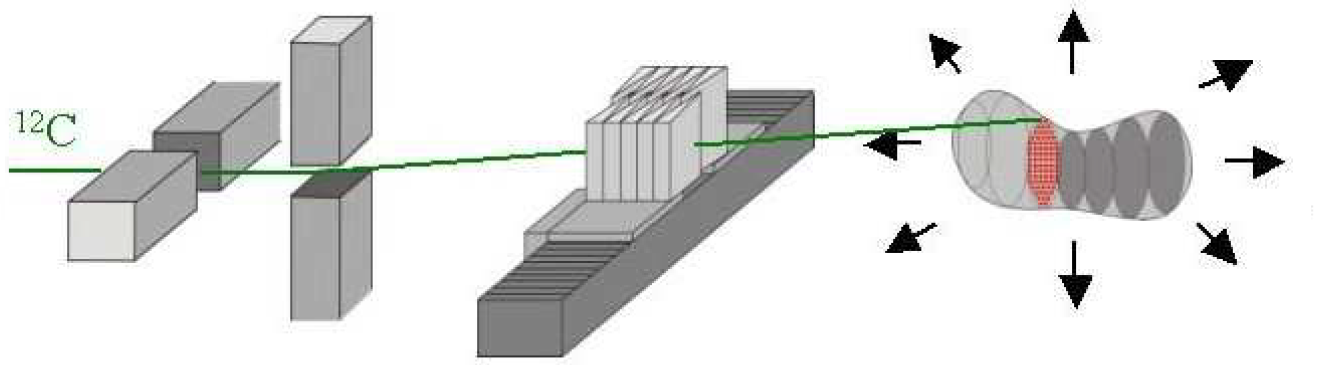
\includegraphics[scale=0.4]{./teile/introduction/tracking.png}
\caption{Principle of tracking at GSI. The lateral deflection is achieved via dipole scanner magnets. For the longitudinal adaptation two 
PMMA wedges are mounted on step motors, enabling to change the depth the particle beam has to traverse. Figure taken from \cite{Gro04}}
\label{tracking}
\end{center}
\end{figure}

Besides these major motion mitigation techniques, different combinations are currently studied. A combination between rescanning and 
gating is e.g. studied by Furukawa et al. \cite{Fur07} or Seco et al. \cite{Sec09} and a combination of rescanning at tracking 
by van de Water et al. \cite{Wat09}.\newline
\newline
As breathing is the main reason for intrafractional motion in most radiotherapy applications, many different other techniques have been 
investigated to directly mitigate the influence of respiration. An example is abdominal pressure, which has been used in lung 
and liver cancer patients in treatments with photons \cite{Neg01, Hof03} and recently also for scanned carbon ions at HIT (treatment 
of hepatocellular cancer \cite{Com11}). Jet ventilation \cite{Hof03} and apneic oxygenation \cite{RPTC12} are also used to partially or 
completely suppress respiration of the patient. 


\subsubsection{4D Treatment planning at GSI}

In order to account for intrafractional organ motion, time-resolved (4D) treatment planning is needed. The underlying data as well 
as the techniques for 4D treatment planning will be presented for the special case of scanned carbon ion beams at GSI.\newline
\newline
As in the static case, treatment planning for ions is based on CT scans. In the special case of 4D treatment planning, these CT scans are 
time resolved (\textbf{4DCT}s, see section \ref{Motionacq}, Motion acquisition). In order to use the information stored in the 4DCT, an \textbf{image 
registration} needs to be performed. With this a voxel-to-voxel mapping between the reference phase of the 4DCT and all other motion phases is 
gained, hence yielding a spatial correlation between the individual CT phases \cite{Ric13}. Usually, rigid and deformable registration 
methods are distinguished. While rigid registration only contains linear transformation of the original object in all three room dimensions, 
deformable registration also accounts for compression. 
Brock et al. \cite{Bro10} published a multi-institutional study where the accuracy of some of the available registration algorithms is 
presented. It can be stated that registration accuracy of most algorithms is in the order of millimeters, hence in the order of a CT 
voxel size, but is dependent on the image contrast (resulting in less accurate results when the contrast is diminished).

\begin{figure}[H]
\begin{center}
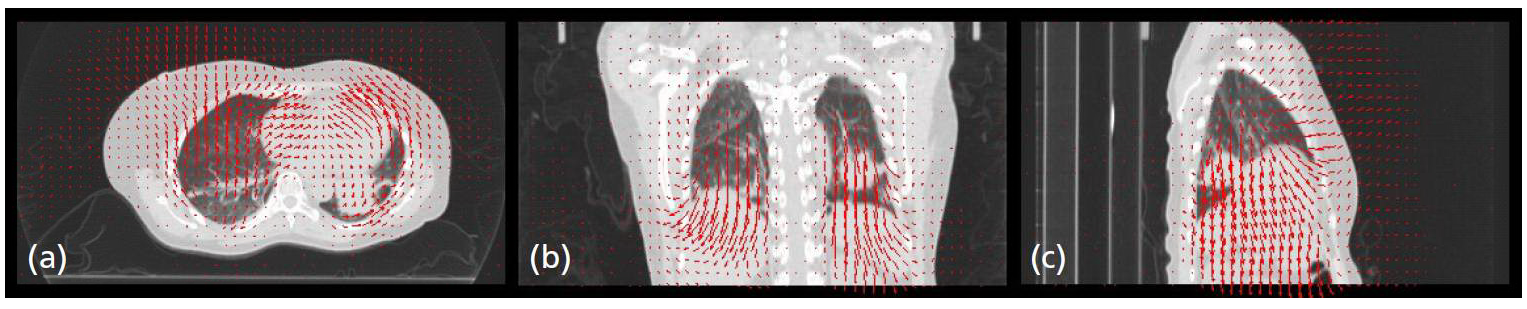
\includegraphics[scale=0.43]{./teile/introduction/registration.png}
\caption{End-exhale, 4D reference phase of a lung cancer patient with overlying deformation field to end-inhale in a) axial, b) coronal and 
c) sagittal view. Figure taken from \cite{Ric12}.}
\end{center}
\end{figure}

\vspace*{-0.8cm}

\textbf{4D treatment planning} at GSI is carried out with the in-house software \textbf{TRiP4D}. It was mainly developed by Daniel Richter \cite{Ric13} and 
is based on TRiP98 as well as a predecessor program developed by Bert and Rietzel \cite{Ber07b} together with the biological implementation 
under influence of target motion by Gemmel et al. \cite{Gem11}.  
TRiP98 was developed for static target regions and was successfully applied in the GSI pilot project \cite{Krae10, Krae00, Krae00b}.  
It is a command-line-based software without graphical interface which runs on an IBM AIX operating system and is written in C 
programming, using a pseudo object-oriented structure. For a detailed description of TRiP4D functionalities as well as of the software 
design and experimental verification the reader shall be referred to \cite{Ric13}. However, a short overview of some of the most important 
functionalities will be given here.\newline
\newline
The \textbf{4DCT structure} was implemented as a sequence of 3DCTs with a distinguished reference CT on which the dose optimization 
process is carried out. Thus the existing 3D functionalities, like the computation of water-equivalent path lengths, could be reused. 
Individual phases of the 4DCT are indexed by their position in the motion cycle. 
TRiP4D does not include native \textbf{image registration} functionalities but rather integrates and processes image registration output, obtained e.g. 
with the open source software package Plastimatch \cite{Sharp07}. The resulting deformation maps need to be obtained in two directions 
(reference-moving and moving-reference) as certain steps of the treatment planning like contour propagation require the inverse deformation 
maps.
\textbf{Contours segmentation}, of target volumes as well as organs at risk, is stored as a volume dataset model, based on the 3D 
segmentation module of TRiP98 with planar polygons on axial CT slices. Based on this 4D segmentation functionality ITVs (see section \ref{tp}) 
can be created, which are needed for certain motion mitigation 
techniques like e.g. rescanning. In general, the 4D treatment plan generation and \textbf{dose optimization} is very dependent on 
the employed motion mitigation technique. For the ITV concept \cite{Gra12}, and hence in motion mitigation techniques where the dosimetric 
effects caused by interplay are compensated but not the target motion itself, dose optimization is carried out on the 4DCT 
reference phase \cite{Ric13}. For beam tracking on the other hand additional optimization is carried out, as motion compensation vectors have 
to be computed. Furthermore 4D optimization techniques (which include the target motion for optimization by using the full 4DCT dataset, the 
vectors from image registration as well as 4DVOIs for dose optimization \cite{Gra13, Ele12}) can be developed and applied with TRiP4D.   
Based on the predecessor program of Bert and Rietzel the \textbf{treatment plan} is then split into quasi-static sub-plans 
where the raster points and the corresponding intensities are divided according to the motion phase they shall be irradiated in. 
For the overall \textbf{4D dose calculation} in TRiP4D, the sub-plans are then collected over all motion states for each dose voxel. Thereby 
the voxel position is transformed according to the deformation maps and by accounting for the radiological density distribution of 
the respective phase of the 4DCT. The total physical dose results as a summation of the dose distribution from all motion states in 
the reference state (see figure \ref{TRiP4Ddose}).  For the biological dose calculation the particle and energy spectra are also accumulated 
over all motion states and used as input for the local effect model (LEM) to calculate the RBE \cite{Scho94, Scho96, Gru12}. 
TRiP4D was extensively tested and verified in numerous experiments \cite{Ric12, Ric13}.  

\vspace*{-0.3cm}

\begin{figure}[H]
\begin{center}
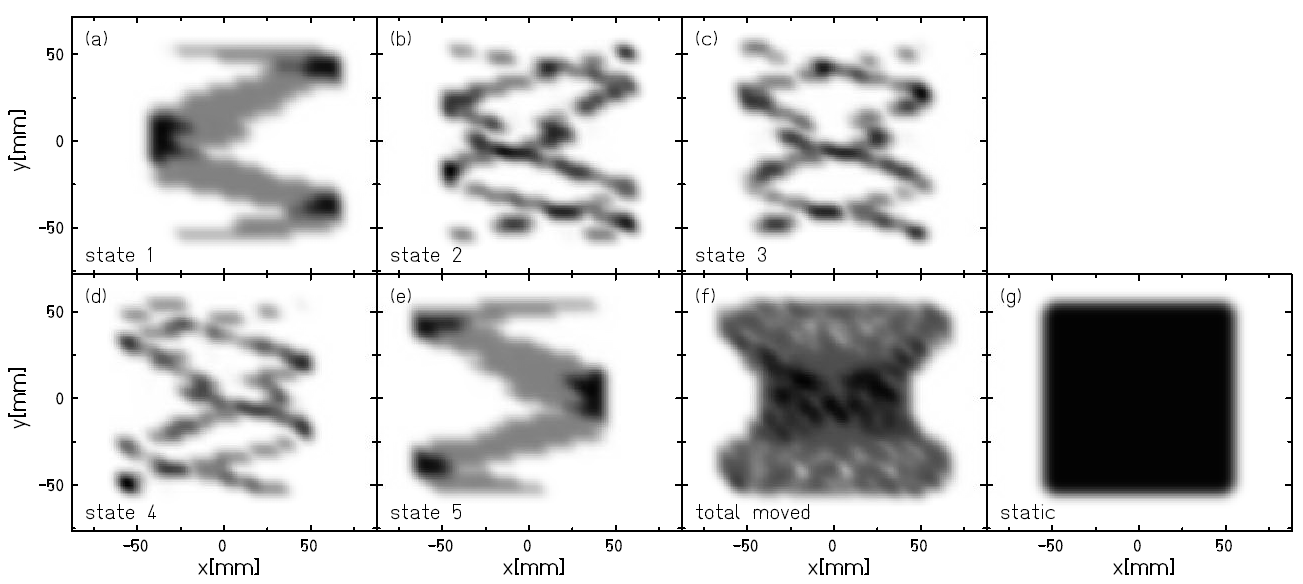
\includegraphics[scale=0.35]{./teile/introduction/4DtreatmentPlanning.png}
\caption{Resulting film response in experimental validation of 4D dose calculation with TRiP4D. Images a)-e) show the individual dose 
deposition in each of the five motion states. In f) the total dose deposition in 4D is displayed. On the stationary film in g) a homogeneous 
dose is deposited in 3D. Figure taken from \cite{Ric12}}
\label{TRiP4Ddose}
\end{center}
\end{figure}



\newpage

%%%%%%%%%%%%%%%%%%%%%%%%%%%%%%%%%%%%%%%%%%%%%%%%%%%%%%%%%%%%%%%%%%%%%%%%%%%%%%%%%%%%
\section{Atrial fibrillation}

Atrial fibrillation (AF) is the most common cardiac arrhythmia. It occurs in $\sim$2\% of the population older than eighty in Europe 
and the US, leading to over six million patients in Europe \cite{ESC10} and over two million patients in the United States \cite{CE09}. The 
lifetime risk of developing AF is $\sim$25\% for people over forty. Since age is an important risk factor for this cardiac arrhythmia the 
prevalence is estimated to double in the next fifty years due to ageing of society (see figure \ref{USincidences}).\newline

\begin{figure}[H]
\begin{center}
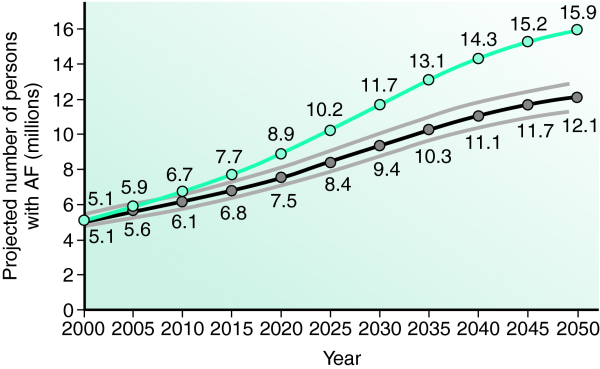
\includegraphics[scale=3]{./teile/introduction/af_incidences_us.png}
\caption{Trend of AF incidences. The black curve indicates the projected number of patients assuming no further increase in age-adjusted AF 
incidences. The green curve represents the trend assuming a continuous increase in incident rates as evident in 1980 to 2000. Figure taken 
from \cite{Miy06}}
\label{USincidences}
\end{center}
\end{figure}

Even though in itself not life threatening, it alters the quality of life and increases the risk to suffer a stroke. It is 
estimated that the stroke risk in AF patients is 5-fold higher \cite{Ben98, Wol91}. AF often remains undiagnosed 
(silent AF). It is stated that one out of five acute strokes is attributed to AF \cite{ESC10}. Other late effects and related events 
include cognitive dysfunctions like vascular dementia and impairment of left ventricular function. In general death rates are stated to 
approximately double by AF \cite{ESC10}, leading to a ten year survival rate of 25\% compared to 46\% in patients with a normal sinus 
rhythm (age ranged from 14 to 73 years with a median of 42 years) \cite{Oles62, ACC06}.\newline
\newline
In the following the normal signal propagation through the heart's conduction system will be explained in order to contrast the occurring 
differences in AF. Possible causes for AF and underlying risk factors as well as current treatment modalities will be presented.

\newpage

\subsection{Heart's conduction system}
\label{HCS}
The conduction system of the heart controls the generation and propagation of electrical signals, so called action potentials, that cause 
the heart muscle to contract and hence to pump blood \cite{Med}. The small electrical activity of the action potentials is measurable at the 
surface of the body, enabling a graphical record with an electronic recording instrument, the Electrocardiograph (ECG). In the following the 
events during a single heart beat and the corresponding detection in an ECG (see fig. \ref{ecg}) will be explained. 
The action potentials can originate spontaneously in any of the specialized cardiac muscle cells which form the conduction system. In a healthy 
heart each beat begins in the right atrium with an action potential from the sinoatrial (SA) node (see fig. \ref{condsys}), making it the 
natural pacemaker of the heart. The signal then spreads across both atrial chambers causing the muscle cells to contract (atrial systole) 
which is represented as the P-wave in an ECG. It is followed by a period of conduction (PR-segment in ECG) in which the signal enters the 
ventricles via the atrioventricular (AV) node. As the signal spreads the ventricles contract very rapidly 
(ventricular systole), which is displayed in the QRS-complex in an ECG. Atrial activity is hidden in the ECG by the QRS complex. As the signal 
passes out of the ventricles, the ventricular walls start to relax (ventricular diastole). The T-wave marks this ventricular repolarization. 
The sequence of these events and the corresponding ECG traces repeat with every single heartbeat.\newline

% \vspace{-7cm}
% \vspace{-1.5cm}
\vspace{-0.5cm}
\begin{figure}[H]
\begin{center}
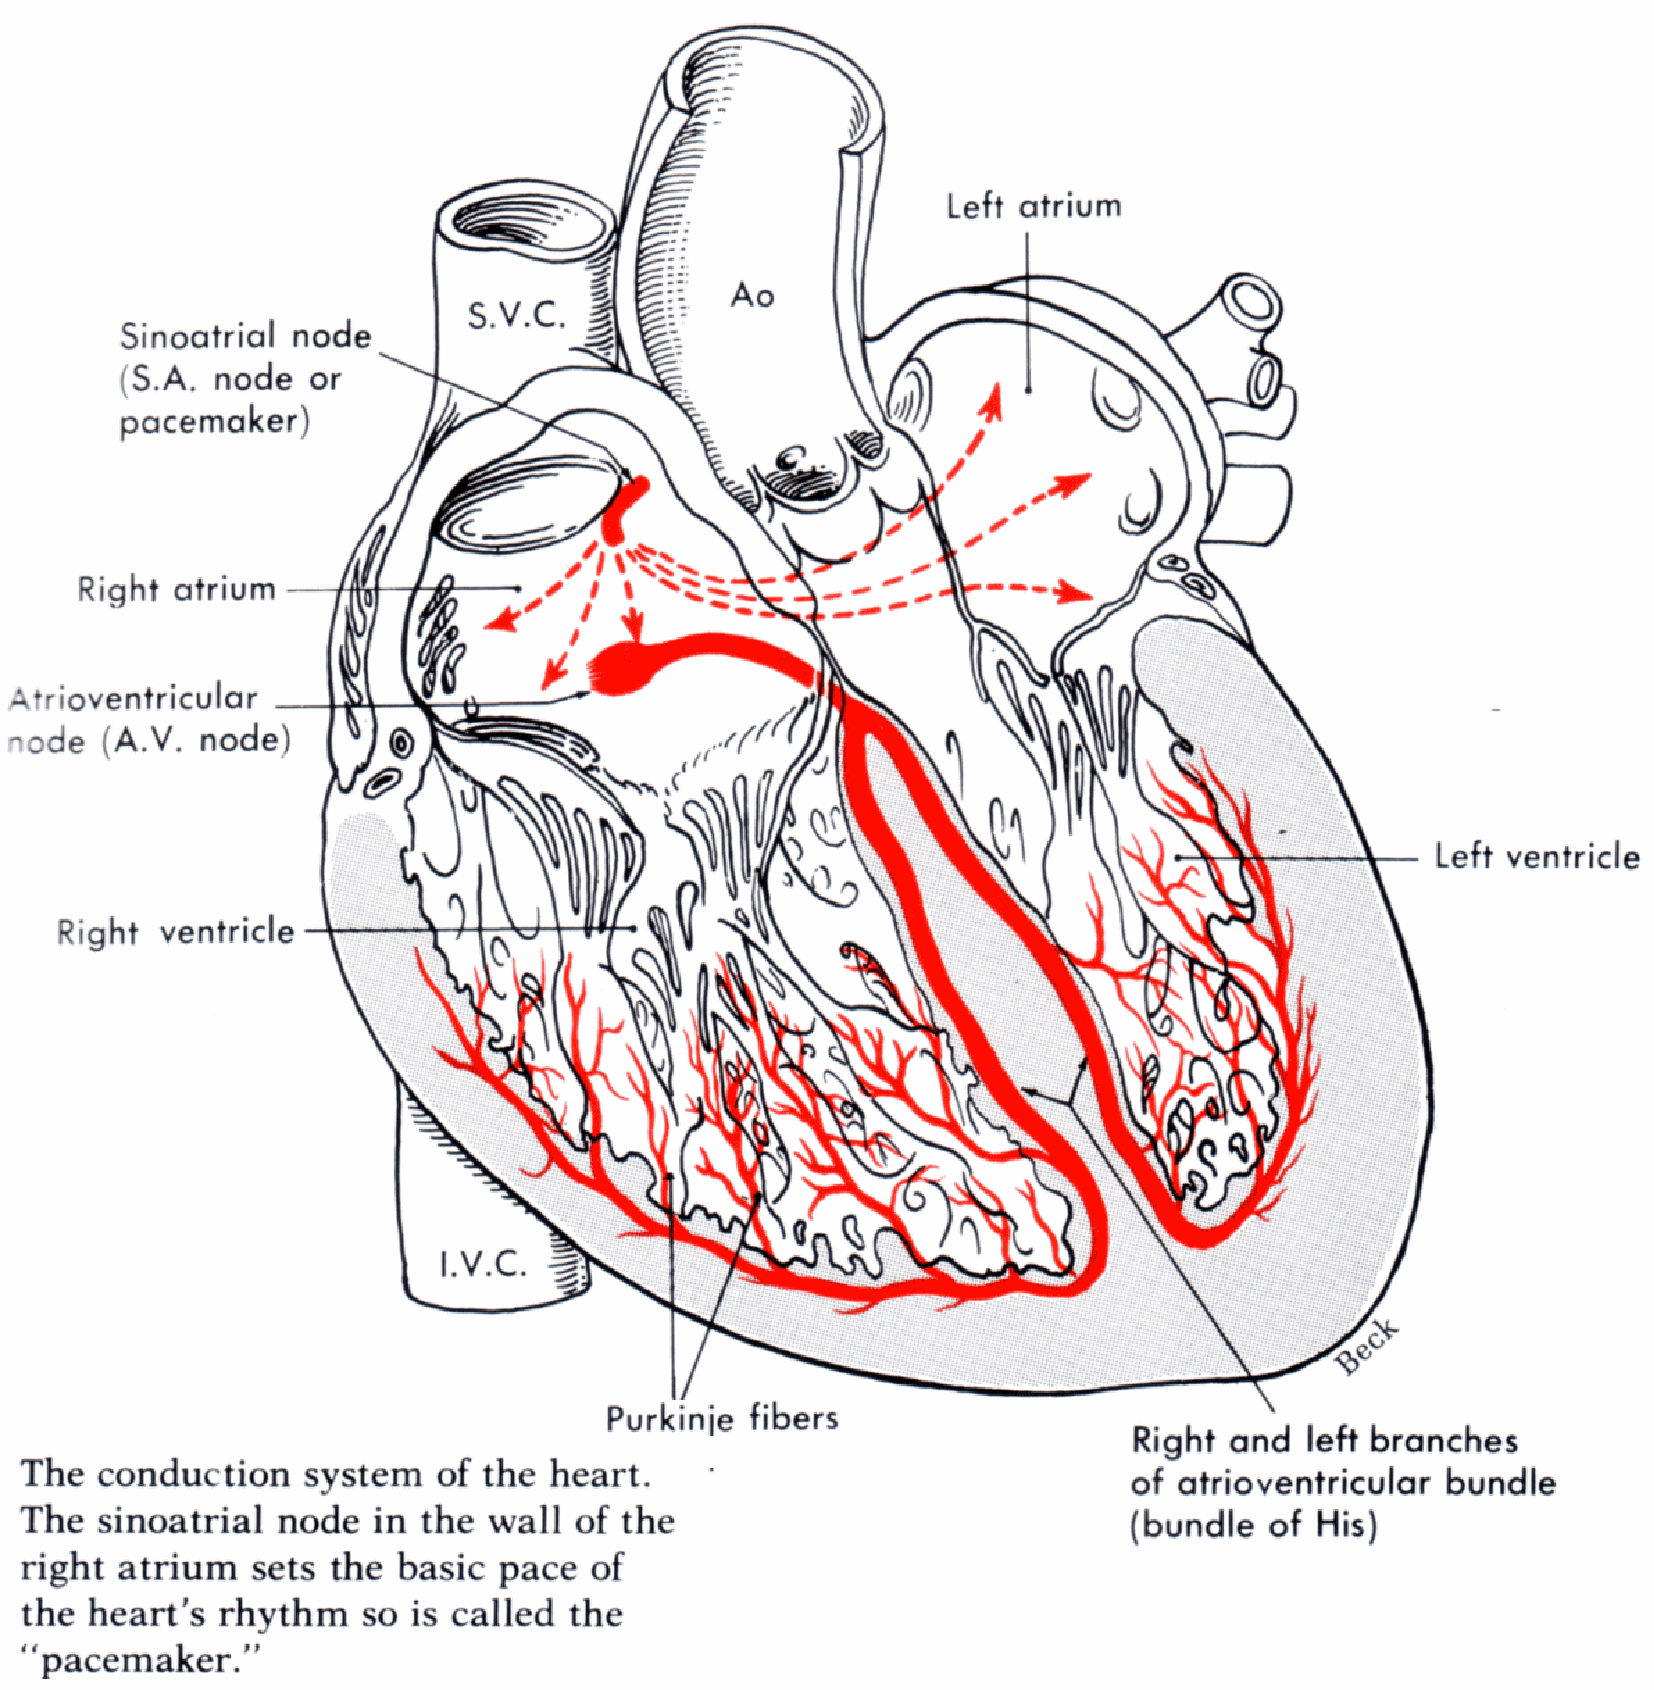
\includegraphics[scale=0.23]{./teile/introduction/conduction_system.png}
\caption{Scheme of the conduction system of the heart. Figure taken from \cite{amc}}
\label{condsys}
\end{center}
\end{figure}

\newpage

\begin{figure}[H]
\begin{center}
% 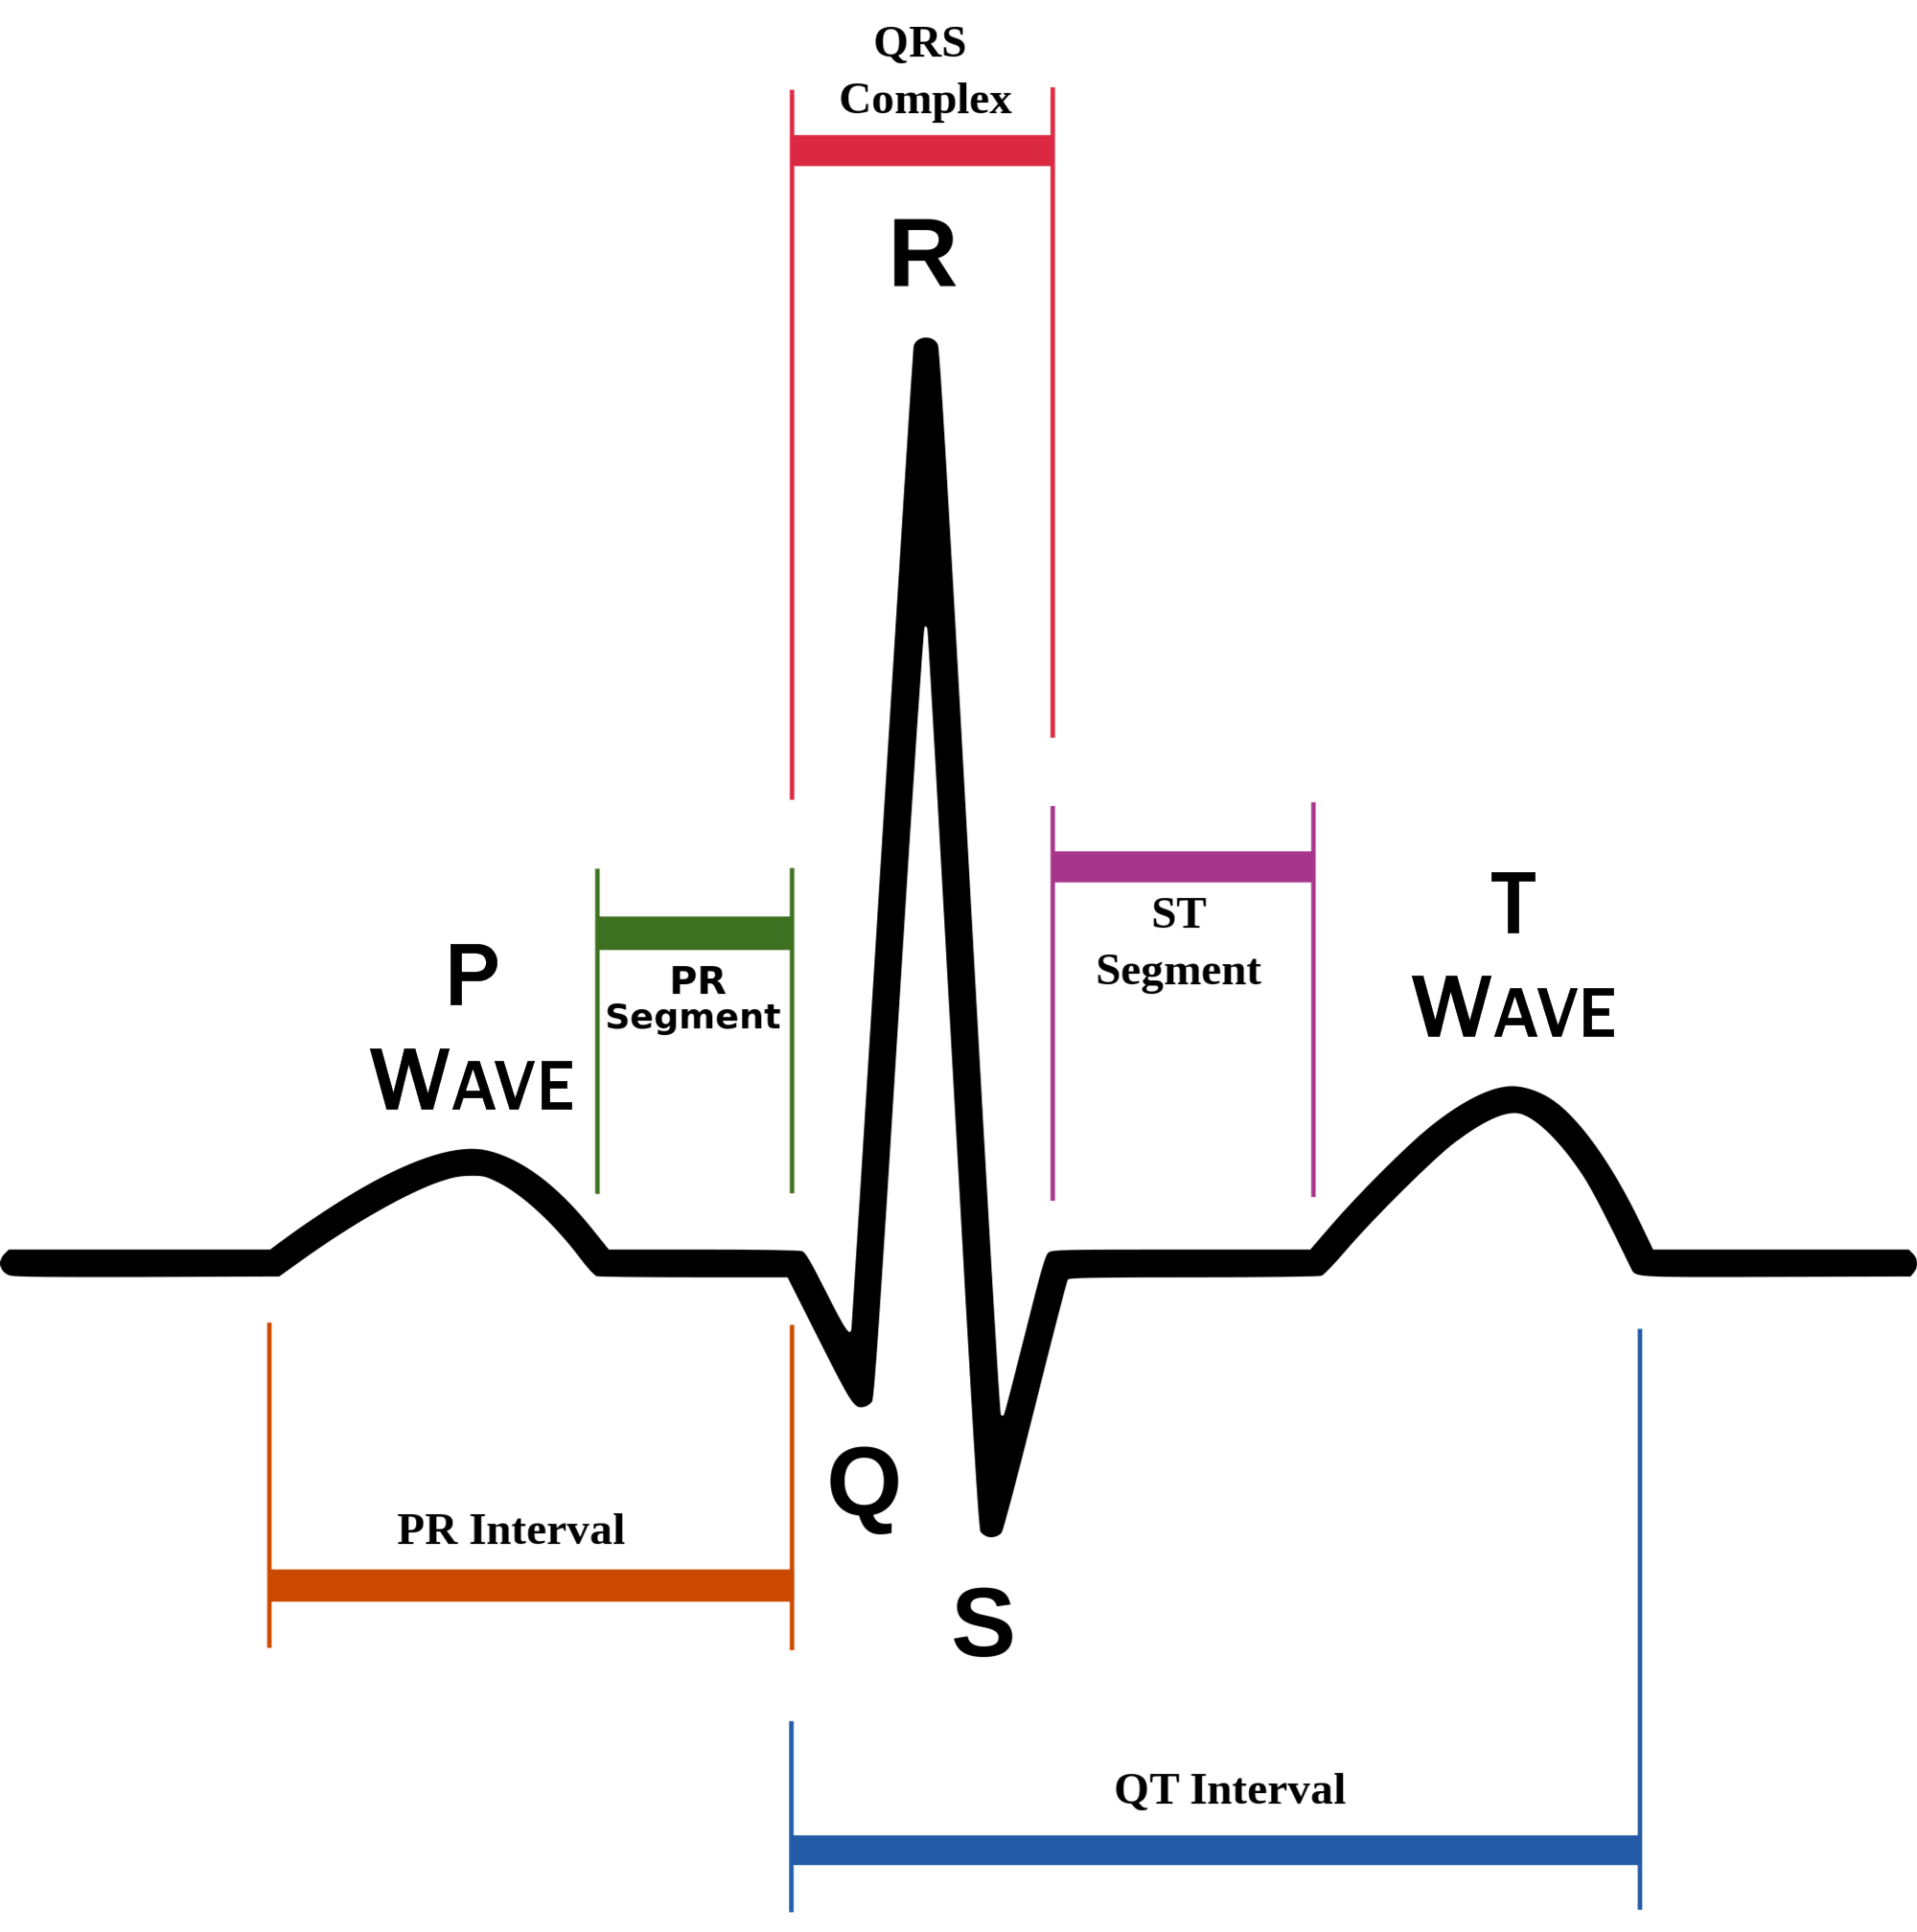
\includegraphics[scale=0.13]{./teile/introduction/ecg.png}
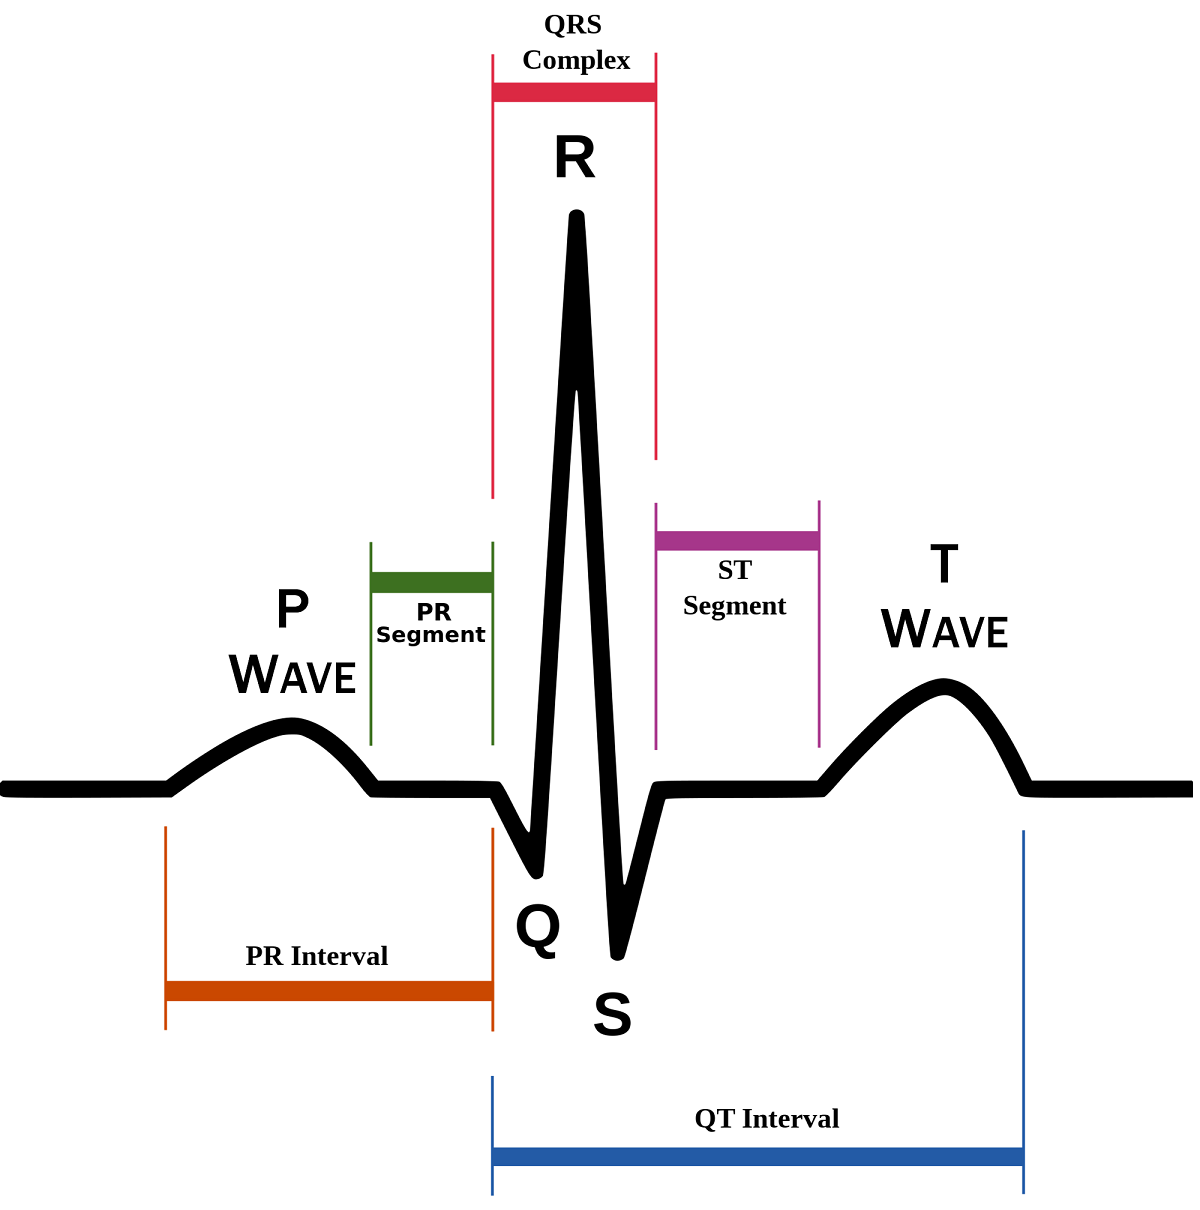
\includegraphics[scale=0.3]{./teile/introduction/ecg_2.png}
\caption{ECG trace of a normal heart beat. Figure taken from \cite{afib}}
\label{ecg}
\end{center}
\end{figure}

In AF there is unorganized atrial activity, leading to quivering motion and hence the atria are not able to sustain a healthy pumping rhythm. 
An exemplary ECG trace for AF can be seen in figure \ref{af_ecg}. 
Possible reasons and triggers for this abnormal action potential propagation are stated in the section \ref{AFriskfactor}.

\begin{figure}[H]
\begin{center}
% 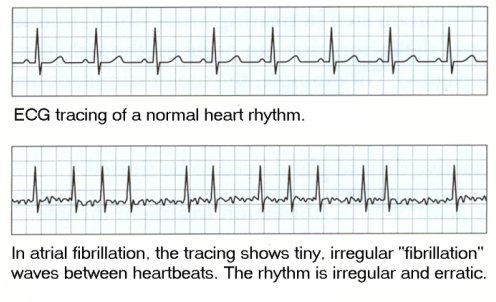
\includegraphics[scale=3]{./teile/introduction/AF_ECG.png}
\subfigure[normal sinus rhythm]{
 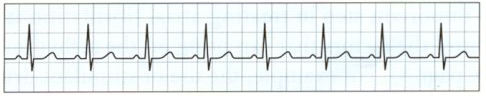
\includegraphics[scale=1]{./teile/introduction/AF_ECG_1.png}
 }
 \subfigure[AF patient]{
 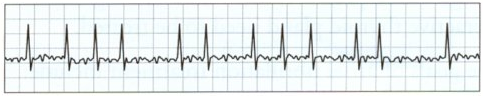
\includegraphics[scale=1]{./teile/introduction/AF_ECG_2.png}
 }
\caption{ECG traces for a normal sinus rhythm (a) and for an AF patient (b). In AF, the tracing shows small, irregular fibrillation waved 
between heartbeats. The rhythm is irregular and erractic. Figure taken from \cite{afib}}
\label{af_ecg}
\end{center}
\end{figure}

\newpage
\subsection{Types of atrial fibrillation}

Based on the duration and presentation of the condition different types of AF are clinically distinguished \cite{ESC10, CE09} (paroxysmal, 
persistent, long-standing and permanent) (see figure \ref{af_types}). Furthermore silent AF may present itself as any form of the stated AF 
types. As the name indicates, the condition is asymptomatic and hence undiagnosed. It usually manifests as an AF related complication like an 
ischemic stroke. About one third of people with AF are estimated to be unaware of their condition \cite{ESC10}.\newline
\newline
Usually AF progresses over time. Starting as short and rare episodes the condition develops into longer and more frequent attacks \cite{ESC10}.
In figure \ref{afovertime} the typical time course of AF is indicated. In the lower part of the diagram different periods of AF are shown 
(dark blue boxes). Possible treatment possibilities at the different stages of AF are shown in the upper bars. Medication uptake which should 
prevent the formation of blood clots are represented by light blue boxes. These medications are recommended in the majority of AF patients. 
The red boxes indicate system relief therapies while the grey boxes represent rate control measures.

\vspace*{0.7cm}

\begin{figure}[H]
% \begin{minipage}{0.475\textwidth}
\begin{minipage}{0.5\textwidth}
\centering
    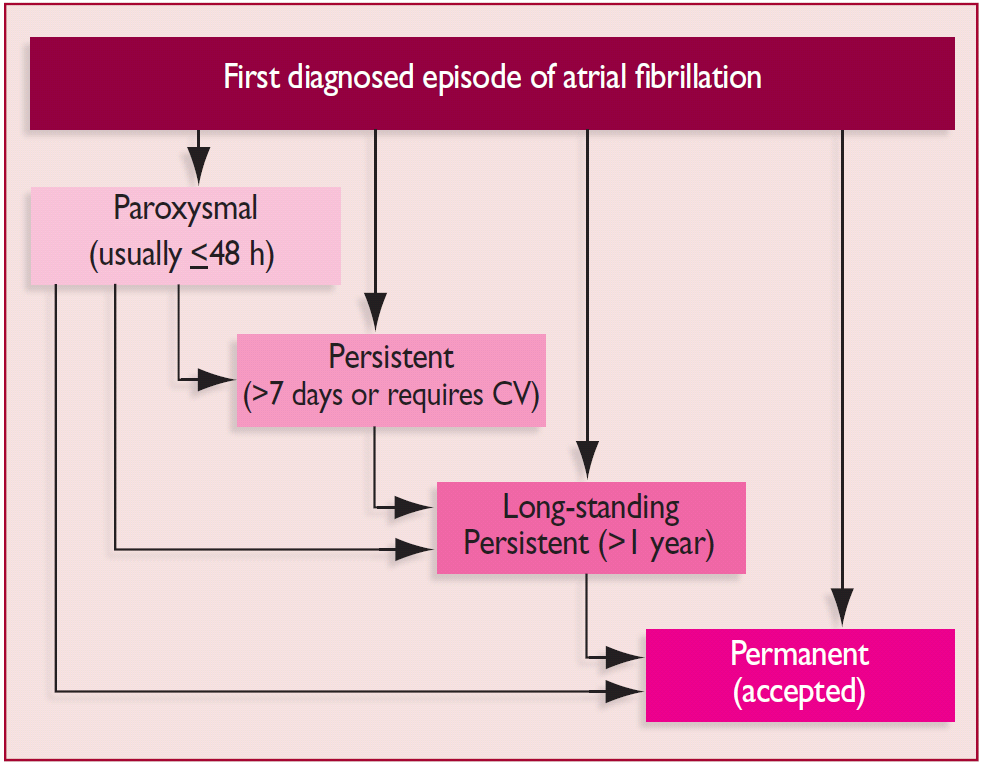
\includegraphics[width=\textwidth]{./teile/introduction/af_types.png}
    \caption{Different types of AF. Figure taken from \cite{ESC10}}
     \label{af_types}
\end{minipage}
\hfill
% \begin{minipage}{0.475\textwidth}
\begin{minipage}{0.52\textwidth}
\centering
  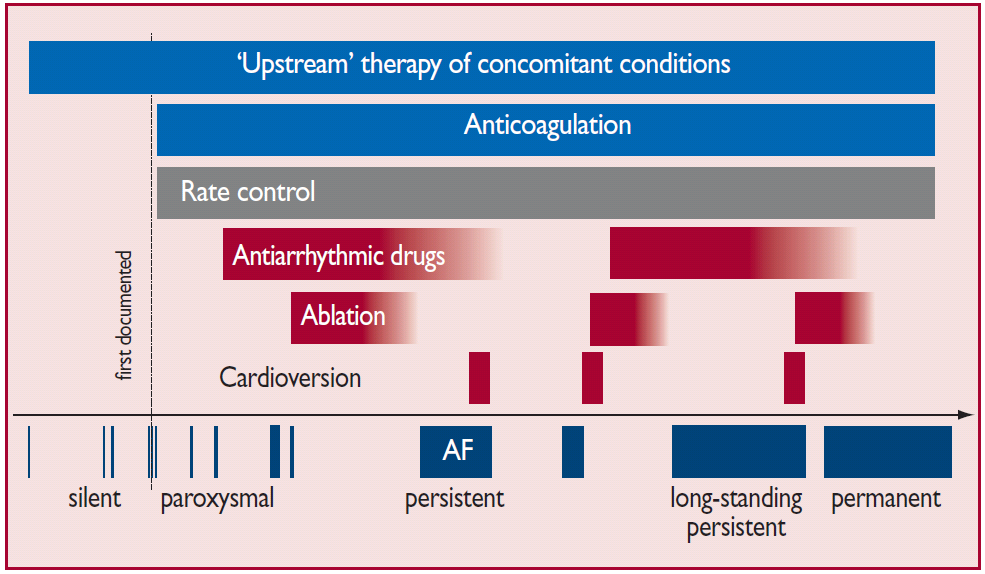
\includegraphics[width=\textwidth]{./teile/introduction/af_over_time.png}
  \caption{Typical time course of AF and potential treatment possibilities. Figure taken from \cite{ESC10}}
  \label{afovertime}
\end{minipage}
\end{figure}

  
% \begin{figure}[H]
% \begin{center}
% 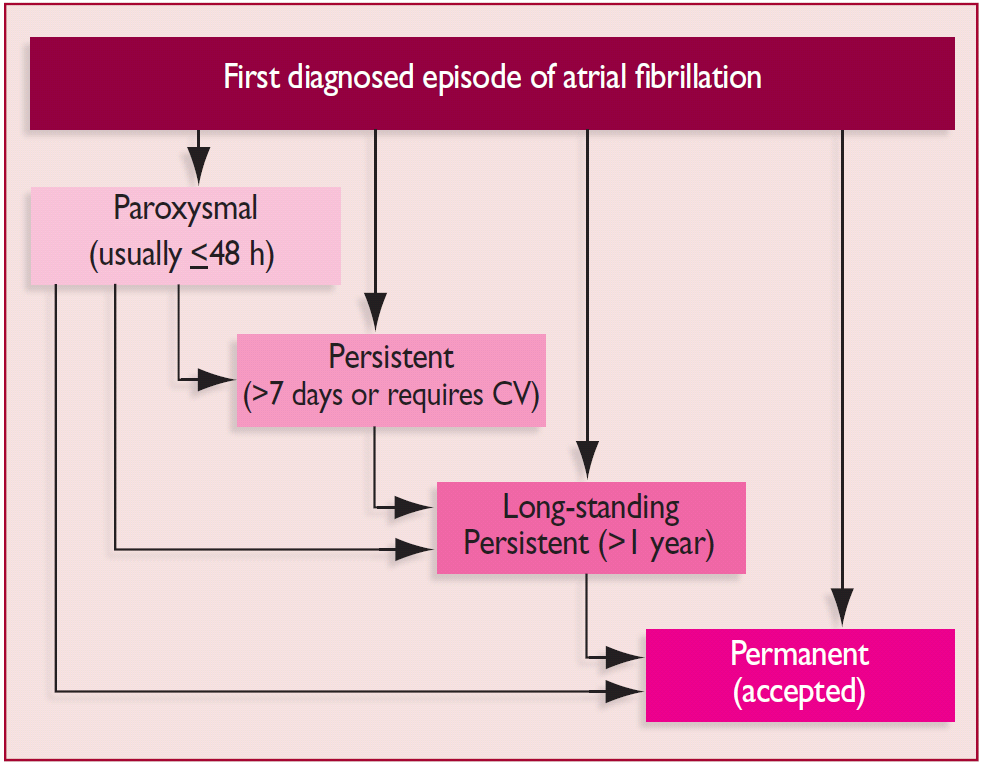
\includegraphics[scale=0.2]{./teile/introduction/af_types.png}
% \caption{Different types of AF. Figure taken from \cite{ESC10}}
% \label{af_types}
% \end{center}
% \end{figure}
% 
% 
% \begin{figure}[H]
% \begin{center}
% 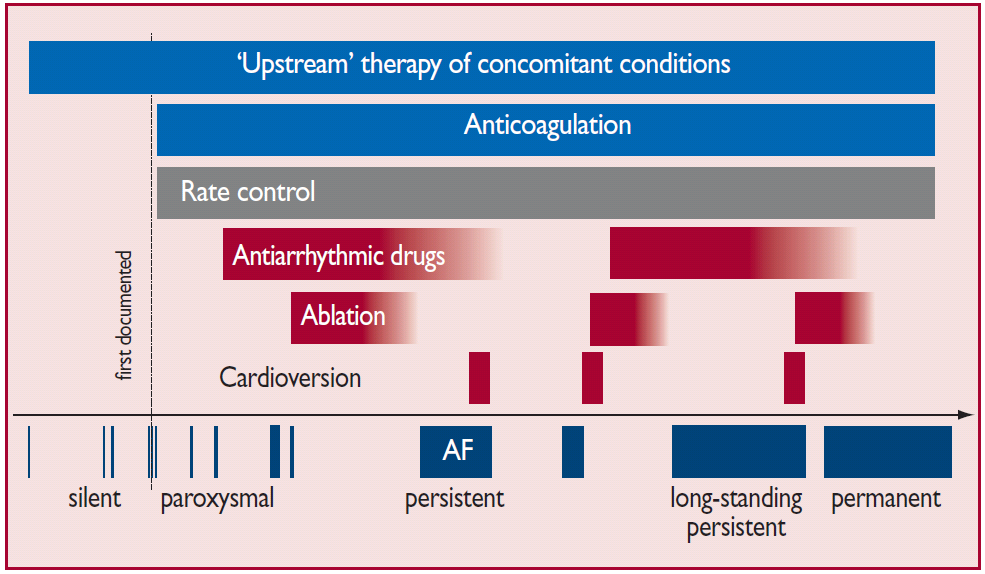
\includegraphics[scale=0.22]{./teile/introduction/af_over_time.png}
% \caption{Typical time course of AF with different periods of AF (dark blue boxes) and possible treatment 
% possibilities as well as medication uptake. Figure taken from \cite{ESC10}}
% \label{afovertime}
% \end{center}
% \end{figure}


\newpage
\subsection{Possible causes for atrial fibrillation and risk factors}
\label{AFriskfactor}

The mechanisms of AF are not yet fully understood. The multifactorial mechanisms may influence and sustain each other. 
Current research indicates that one can distinguish between focal 
mechanisms and multiple wavelets \cite{CE09}. For most patients with paroxysmal AF a localized, focal trigger can be identified. This is 
not the case in patients with persistent or permanent AF, where the multiple wavelet hypothesis is believed to be more accurate.\newline

An identified \textbf{focal trigger} site are the pulmonary veins (PVs). In the benchmark paper Ha\"{\i}ssagurre et al. \cite{Hai98} studied 
45 patients with frequent episodes of AF ( (344 $\pm$ 326)minutes episodes per 24 hours) finding ectopic beats\footnote{beats which arise 
from cells outside the region in the heart muscle ordinarily responsible for impulse formation} originating from the pulmonary veins in 
94\% of the cases. The underlying mechanism why PVs become arrhythmogenic in some patients while it remains dormant in others is 
still not clear \cite{CE09}. The reason why PVs can become arrhythmogenic at all is based on stages during the embryonic development, in 
which the common PV is incorporated into the left atrium. Immunohistochemical studies have shown that the composition of the PV and the 
smooth-walled portion of the left atrium are identical (see figure \ref{walls}) \cite{CE09, Doug06}. 

\vspace*{-0.5cm}
\begin{figure}[H]
\begin{center}
% \includegraphics[scale=4.0]{PVatriumTissue.png}
\includegraphics[scale=3.5]{./teile/introduction/PVatriumTissue.png}
\caption{Schematic depiction of outer side of atrial chambers with pulmonary veins (PV), left atrial appendage (LAA), left atrial body (LAB), 
right atrial body (RAB), superior vena cava (SCV) and inferior vena cava (IVC). LAB and RAB are covered by myocardium (heart muscle tissue) 
with smooth-walled inner aspect (blue), which stretches out over extra cardiac segments of PV (blue area above and below dotted line). 
In A the structures are illustrated from the outside, while B shows the tissue types from the inside of the atria. Figure 
taken from \cite{Doug06}}
\label{walls}
\end{center}
\end{figure}

\vspace*{-0.6cm}
Furthermore, according to the \textbf{multiple wavelet hypothesis} AF is sustained by the continuous propagation of several independent 
wavelets \cite{CE09}. These wavelets are propagating through the muscles of the atria in a chaotic manner. Interference effects between 
various wavelets lead to amplification or cancellation. As long as the number of wave fronts does not decline a certain threshold level AF 
is sustained.\newline

Certain risk factors and indicators for AF can be found in the AF patient group \cite{CE09}. Ageing generally increases the risk of 
developing AF. The reason might be due to age dependent loss of atrial myocardium and the associated conduction disturbances. Hypertension 
is also an age dependent factor which is a risk factor for the incidence of AF as well as AF-related complications such as stroke and 
systematic thromboembolism. Thyroid dysfunction
can be the sole cause of AF and may induce AF related complications. 25\% of AF patients are obese \cite{Nab09} and 20\% suffer of 
diabetes mellitus requiring medication. Chronic obstructive pulmonary 
disease (COPD) is found in (10 - 15)\% of AF patients. Nevertheless it is possibly more a marker of general cardiovascular risk then an 
indicator for AF. Chronic renal disease is present in (10 - 15)\% of AF patients and it is suggested that renal failure may increase the 
risk of AF related complications \cite{CE09}. Independent of the stated risk factors AF has also a genetic component, especially 
considering an early onset of AF. In a study carried out by Fox et al. \cite{Fox09} with 2243 offspring participants it was stated that the 
risk of developing AF compared to no parental AF was significantly increased (multivariable-adjusted odds ratio of 1.85, 95\% confidence 
interval). The results were even stronger when age was limited to an age younger than 75 in parents as well as their offspring 
(multivariable-adjusted odds ratio of 3.23, 95\% confidence interval). 


\subsection{Treatment modalities}

The treatment modalities for AF have two main goals: to reset the rhythm or to control the ventricular rate and to prevent the formation of blood 
clots \cite{Mayo, CE09}. The treatment strategy chosen for each individual patient depends on the type of AF and on careful 
consideration of patient individual factors, including the severity of symptoms and potential further heart problems. \newline

Resetting the heart rhythm is the ideal treatment outcome and is carried out by cardioversion, either based on medication (anti-arrhythmic 
drugs) or electrically. In an electrical cardioversion an electrical shock is delivered to the heart, giving the conduction system of the 
heart the possibility to restore its normal activity. Commonly used anti-arrhythmic drugs are e.g. Amiodarone. These drugs have severe side 
effects and can act proarrhythmic, causing also life-threatening ventricular arrhythmias \cite{Mayo}.\newline

If AF can not be converted to a normal heart rhythm through the above stated methods, the ventricular rate needs to be reduced instead. 
Heart rate control can be achieved either by the usage of different medication (e.g. Lanoxib) or by AV node ablation.  
This procedure requires simultaneously the implementation of a pacemaker to establish a heart beat. Hence the atria are still 
fibrillating, further medication with anti-arrhythmic medication as well as anticoagulants is required.\newline

For paroxysmal or persistent AF further treatment modalities are needed. They include the \textbf{Maze procedure} or \textbf{radiofrequency catheter ablation}.\newline

In the \textbf{Maze procedure} scar tissue in the atria is created, inhibiting the propagation of abnormal action potentials. Similar to a maze, 
only a single pathway from the the SA node to the AV node remains accessible for electrical impulses \cite{CTS13}. 
Besides an open chest surgery, the Maze procedure can also be carried out as minimal-invasive procedure or as cryotherapy. The success rates as well as 
complications of Maze versus catheter ablation will be described in the next section.\newline


In \textbf{catheter ablation} the main strategy is anatomic based, which means that it is assumed that AF is triggered and sustained by the 
same anatomical sites (the PVs \cite{Hai98}) in the majority of AF patients \cite{CE09}. In radiofrequency ablation a flexible catheter is 
inserted into the patient through a vein close to the groin of the patient and threaded into the heart. An electrode on the tip of the catheter 
sends out radiofrequency waves, creating energy and thus heat. This is used to create a 
scar close to the junction between the pulmonary veins and the atria (see figure \ref{af_circ}).\newline

\vspace*{-0.6cm}
\begin{figure}[H]
\begin{center}
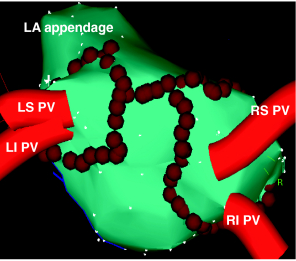
\includegraphics[scale=0.7]{./teile/introduction/ablation_cut.png}
\caption{Example of circumferential PV ablation. The ablation sites are indicated by the red dots. LI PV: Left inferior pulmonary veins, 
LS PV: left superior pulmonary veins, RI PV: right inferior pulmonary veins, RS PV: right superior pulmonary veins. Figure adapted 
from \cite{Ora06}}
\label{af_circ}
\end{center}
\end{figure}

\vspace*{-0.7cm}

Various ablation techniques exist, including the PV isolation by segmental ostial ablation, circumferential PV ablation (see 
fig. \ref{af_circ}), wide-area circumferential ablation and antral PV isolation \cite{Ora06, Ora03, Ouy04}. Antral PV isolation 
and wide-area circumferential ablation was shown to be effective for both patients with paroxysmal and persistent AF \cite{CE09, Ora03}. 
In a randomized study circumferential PV ablation was found to result in a sinus rhythm in 74\% of patients with chronic AF \cite{Ora06}. \newline

\newpage

The goal of PV ablation is to induce a complete electrical isolation of the PVs. This is verified by entrance and exit block during 
pacing at multiple sites within the PVs \cite{CE09}. Freedom from recurrent AF can be predicted by 
termination and noninducibility of AF during catheter ablation \cite{Ora02, Ora06, Hai05, Hai04, Ora04}. Termination 
of AF indicates elimination of all triggers and drivers of AF while noninducibility indicates the absence of residual trggers and drivers 
that may initiate and perpetuate AF \cite{CE09}. Termination is hence not a reliable predictor in patients with paroxysmal AF while 
noninducibility is likely to predict that the patients are going to stay in sinus rhythm (see figure \ref{freedom_recurrence}). 

\begin{figure}[H]
\begin{center}
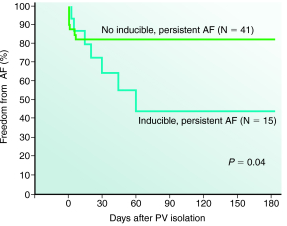
\includegraphics[scale=1]{./teile/introduction/freedom_recurrence_AF.png}
\caption{Graph showing freedom from AF reocurrence when patients had or had not inducible AF after circumferential PV isolation. Figure adapted 
from \cite{Ora04}}
\label{freedom_recurrence}
\end{center}
\end{figure}

% \newpage

\vspace*{-0.4cm}

Independent of the used procedure, anticoagulants like Warfarin are used in a diversity of patients. In order to establish international 
criteria for risk patients who should uptake anticoagulants, the CHADS$_{2}$-VASc score was defined \cite{ESC12} 
(\textbf{C}ongestive heart failure: 1 point, \textbf{H}ypertension: 1 point, {A}ge ($\geq$ 75): 2 points, \textbf{D}iabetes mellitus: 1 point, 
\textbf{S}troke: 2 points, \textbf{V}ascular disease: 1 point, \textbf{A}ge (65-74): 1 point, \textbf{S}ex (female): 1 point). 
Patients who obtain at least 2 point in the CHADS$_{2}$-VASc score are prescribed anticoagulants. Patients with 1 point might be prescribed 
anticoagulants, alternatively aspirin can be used. Patients with a score of 0 are supposed to only take aspirin \cite{Fle}. The 
CHADS$_{2}$-VASc score has been validated in multiple cohorts \cite{Lip11, Pot12, Ole12, Van11, Fri12, Ole11, Bor11}.


\newpage

\subsubsection*{Catheter ablation of AF: success rate and complications}

The FAST trial compared the outcome of catheter ablation and surgical ablation in a randomized study with a small patient population of 127 
patients. 63 patients were treated with catheter ablation, 64 with the invasive surgical ablation. 
The complication rate in catheter ablation was significantly lower (15.9\% complication rate in catheter ablation versus 34.4\% in surgical 
ablation) but at the same time the success rate in treatment outcome was reduced (36.5\% for catheter ablation versus 65.6\% for surgical 
ablation after 12 months) \cite{Boe12}. \newline

In two nationwide surveys the success rates of catheter ablation as a treatment for AF and the resulting complications were studied \cite{Cap05, Cap10}. 
The first worldwide multicenter survey was published in 2005 using data obtained from 181 centers in-between 1995 and 2002. 
From these centers 90 stated to have performed 12,830 catheter ablation procedures on 8,745 AF patients. 
It was stated that 52\% of AF patients undergoing ablation were symptom free without the need of further antiarrhythmic medication and 23.9\% 
of patients with the need of antiarrhythmic drugs. These success rates were achieved with the requirement of a 
a second (in 24.3\% of patients) or even third (in 3.1\% of patients) procedure \cite{Cap05}. Major complication rates were reported in 
6\% of patients. These complications included 4 early deaths (due to massive cerebral thromboembolism in two patients, extrapericardial PV 
perforation in one patient and unknown reasons in one patient), strokes (in 20 patients), transient ischemic attacks\footnote{"mini-stroke"; stroke-like symptoms due to loss of blood flow, no permanent damage} 
(in 47 patients) and episodes of tamponade\footnote{fluid collects between the heart muscle and the pericardium, which is the sac containing 
the heart} (in 107 patients). 
In a second survey which was performed in-between 2003 and 2006 \cite{Cap10} and included 85 catheter ablation 
performing centers (16,309 patients), an improvement in treatment outcome was shown. 
The rate for a successful treatment outcome without the need of further antiarrhythmic medication increased to 
70\% while the rate with the need of further antiarrhythmic medication decreased to 10\%, resulting in an overall success rate of 80\% 
compared to 75.5\% in the first survey. Concerning the number of needed procedures it was stated that 37.1\% single treatments were performed, 
59.8\% dual treatments and 4.1\% triple treatments.\newline

Recent studies furthermore show that catheter ablation procedures in AF patients are associated with a 
substantial risk of developing silent cerebral embolism \cite{Her13, Gai10, Marti13, Med13, Schr10, Lic06}. 
Silent cerebral embolism can cause cognitive impairment \cite{Kne08}. A study by Medi et al. \cite{Med13}, which investigated the 
post-operative neurocognitive dysfunction in 150 patients undergoing ablation before and after the treatment, stated a 13\% - 20\% incidence 
at long-term follow up of 3 months compared to a control group. \newline

Besides these major complications general disadvantages in the treatment modality of catheter ablation can be concluded. 
Procedures are tedious and can take up to five hours \cite{Jong05}. As fluoroscopy is still the mainstay of catheter imaging in most 
laboratories the patients are furthermore exposed to relatively high X-ray dose \cite{Ber10}. From an socio-economical point of view, 
catheter ablation causes high costs. A total of 13.5 billion Euro are spent on AF patients each year in the EU \cite{Fus06}.\newline

It can be concluded that catheter ablation offers only a limited treatment success rate while major complications and even death due to the 
procedure may occur. Alternative treatment modalities are warranted. Catheter-free ablation using carbon ions could have the potential to 
accurately eliminate arrythmogenic sources at any given cardiac location. So far conducted studies to irradiation of cardiac target sites will 
be presented in the next section. 


\subsubsection*{Heart irradiation and cardiac radiosurgery}
\label{cardiacradiosurgery}

Target sites in the heart have been irradiated in different procedures. Re-stenosis\footnote{reoccurrence of blood vessel narrowing} after 
angioplasty\footnote{mechanical widening of narrowed blood vessel e.g. with a balloon catheter} for example has been treated with vascular 
brachytherapy \cite{Nat99, Cot05}. Thereby a minimum dose of (8-16)Gy to a depth of 0.5mm into the vessel wall was required, while a 
maximum vessel dose did not exceed 32Gy. Cardiac angiosarcoma, a very rare tumor type in the heart with rare long-term 
survival of the patients, has been treated with carbon ions at the Japanese facility NIRS \cite{Aok04}. A total dose of 64Gy was given in 16 
fractions in a timeframe of 4 weeks. Follow-up of one and a half year did not show severe side effects.\newline
\newline
Similar to the techniques used in vascular brachytherapy, P\'erez-Castellano et al. \cite{Per06} studied the possibility to use $\beta$-radiation 
as treatment modality for AF. They thereby used a phosphorus-32 source wire centered within a balloon catheter in a study with ten mini swine. 
The delivered dose was calculated to 60Gy at a depth of 1 mm from the contacting PV wall, resulting in observed PV fibrosis without PV stenosis 
or other side-effects.\newline
\newline
In 2010 a study by Sharma et al. \cite{Sha10} showed that they were able to successfully alter the electrical pathway of the heart 
noninvasively by using stereotactic robotic radiosurgery. In the CyberHeart system cardiac target sites in sixteen mini swine were irradiated 
under general anesthesia. The procedure was as follows. Cardiac CT scans of the anesthetized and intubated mini swine were acquired and an 
electroanatomic mapping\footnote{CARTO system; Biosense-Webster. Three known magnetic sources are used to calculate the orientation 
and position of the catheter tip in 3D, while at the same time the voltage values are determined \cite{bw}} was carried out before the 
irradiation. The voltage was mapped to enable a comparison with the later to be induced electrophysiological effect. Different target sites 
in the heart were chosen. The respiratory motion was compensated by tracking with the CyberKnife Synchrony software, which correlates the 
outside motion of radiopaque markers on the chest wall with the internal motion 
\cite{Ozh08}. For the cardiac motion an ITV approach was chosen. Target volumes were the cavotricuspid isthmus (CTI) (nine mini swine), 
the AV node (two mini swine), the pulmonary vein - left atrial junction (three mini swine) and the left atrial appendage (two mini swine). 
Dose ranges from 25Gy to 80Gy were applied (cavotricuspid isthmus: (25-80)Gy, AV node: (40-70) days, PV: (38-40)Gy and left atrial 
appendage: (32-80)Gy). Post irradiation the mini swine were stored at a farm. The follow-up time was dependent on the irradiated target in 
the mini swine (cavotricuspid isthmus: 25 to 89 days, AV node: 15 to 49 days, PV: 35 to 196 days and left atrial appendage: 16 to 33 days). 
In order to assess the irradiation outcome, the animals were again anesthetized and electroanatomically mapped. Afterwards the mini swine 
were euthanized and targets (heart) as well as organs at risk (lung, esophagus) were excised and fixed in formaldehyde. The results of the 
irradiation can be summarized as follows:
The irradiation of the cavotricuspid isthmus evolved during the study, leading to changes in the method of targeting. While initially the 
respiratory and cardiac motion were not compensated for, synchrony and cardiac ITV concepts were later used. While all mini swine 
displayed a reduced conduction across the isthmus, only two animals showed bidirectional block and hence feasibility at 30 days and 40Gy.   
Targeting the AV node, one animal had to be sacrificed due to pacemaker pocket infection. The other one showed a complete AV block at 49 days, 
after being irradiated with 70Gy. For the left atrial appendage a decreased voltage was observed at 38Gy after 33 days. For the left 
pulmonary vein the feasibility was shown as the left atrium showed no local activation in all animals (present from day 35 for all doses) 
(see figure \ref{LA_map}).

\begin{figure}[H]
\begin{center}
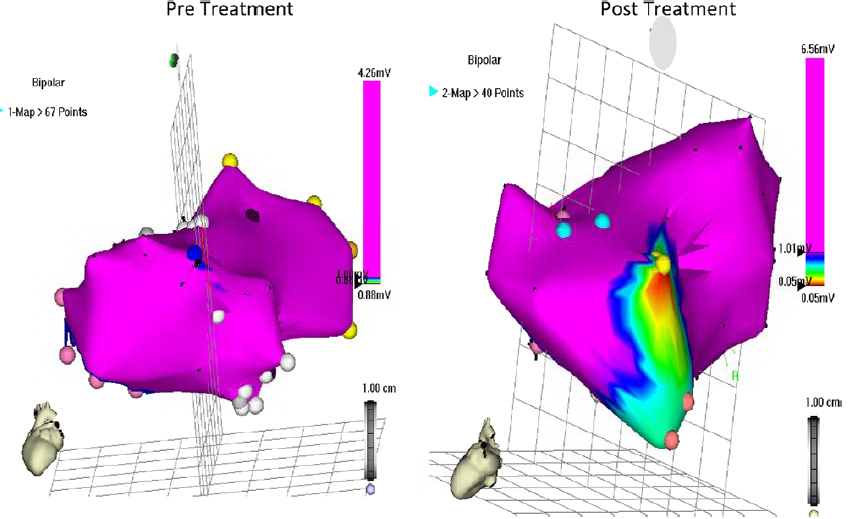
\includegraphics[scale=0.45]{./teile/introduction/cyberheart_voltagemap.png}
\caption{Electroanatomic voltage map of left atrium before (left side) and after (right side) CyberHeart irradation of PVs. Prior treatment 
no decreased voltage can be observed. Post treatment an area of low-amplitude action potential signals can be seen. Figure from \cite{Sha10}}
\label{LA_map}
\end{center}
\end{figure}

Sharma et al. stated that a dose of 25Gy or larger was needed to see a change in the electrophysiological properties in the animal model 
after 30 or more days. The dose needed for myocardial fibrosis is also known from other former studies. Fajardo et al. \cite{Faj70, Faj73} for 
example studied radiation induced fibrosis in rabbit hearts. They observed myocardial fibrosis most often after 2 to 70 days when irradiating 
the rabbits with 20Gy. Overall Sharma et al. proved that stereotactic radiosurgery has the potential to become a noninvasive treatment 
modality for e.g. atrial fibrillation. \newline

A subsequent study carried out with the CyberHeart system \cite{Mag11} only targeted the pulmonary veins atrial junction. Two mini swine 
were irradiated with a single fraction treatment of 25Gy and 35Gy, respectively and followed for 6 months. It was stated that both animals 
showed circumferential fibrosis, leading to an electrical isolation of the PVs, which was detected with an electroanatomic mapping. 
The mini swine irradiated with 35Gy showed more extensive necrosis and vasculitis in intramyocardial vessels. It was hence implied that 
25Gy are sufficient to induce a PV isolation with no major complications in the studied timespan. \newline

In an animal study carried out by Blanck et al. \cite{Bla13} 8 mini swine were irradiated with a single fraction of seven fields with doses 
between 17.5Gy and 35Gy. A 5D-ITV concept was applied, hence applying internal margins to the upper right PV accounting for the respiratory 
and heartbeat. Prior treatment electroanatomic mapping was carried out. The animals were followed for 6 months. In this study it was stated 
that a reduction of the electrical signal procession with correlating local transmural fibrosis in the target region was observed at 
doses above 30Gy. Nevertheless a complete block of the PVs could not be achieved. Stenosis in one branch of 
the PV was observed for the highest applied dose.\newline

All these studies were carried out with photon irradiation. Due to the physical and biological properties of carbon ions (see section \ref{pbb}) 
an improved outcome is expected when treating these deep seated target volumes while sparing the critical organs close by and exposing 
less volume of myocardium to low dose of radiation \cite{Ber12}. The feasibility of this treatment modalities with scanned carbon ions is the aim of 
the present work. 


                                                                                                                                                                                                                              
% \end{document}
